\RequirePackage{fix-cm}
\documentclass[11pt,a4paper,twoside]{vutinfth}

% useful packages
\usepackage{graphicx,textpos}
\usepackage{float}
\usepackage{helvet}
\usepackage{lettrine}
\usepackage{lipsum}
\usepackage{amsmath}
\usepackage{fancyhdr}
\usepackage{multicol}
\usepackage{setspace}
\usepackage[super, numbers]{natbib}
\usepackage{emptypage}
\usepackage[linktocpage=true]{hyperref}
\usepackage[toc,acronym,nonumberlist]{glossaries}
\usepackage{tocloft}
\usepackage{wrapfig}
\makeglossaries

% Import packages for drawing diagram
%More defined colors
\usepackage[dvipsnames]{xcolor}
% Required package
\usepackage{tikz}
\usetikzlibrary{positioning}

% Load packages to allow in- and output of non-ASCII characters.
\usepackage{lmodern}        % Use an extension of the original Computer Modern font to minimize the use of bitmapped letters.
\usepackage[T1]{fontenc}    % Determines font encoding of the output. Font packages have to be included before this line.
\usepackage[utf8]{inputenc} % Determines encoding of the input. All input files have to use UTF8 encoding.

% Extended LaTeX functionality is enables by including packages with \usepackage{...}.
\usepackage{amsmath}    % Extended typesetting of mathematical expression.
\usepackage{amssymb}    % Provides a multitude of mathematical symbols.
\usepackage{mathtools}  % Further extensions of mathematical typesetting.
\usepackage{microtype}  % Small-scale typographic enhancements.
\usepackage[inline]{enumitem} % User control over the layout of lists (itemize, enumerate, description).
\usepackage{multirow}   % Allows table elements to span several rows.
\usepackage{booktabs}   % Improves the typesettings of tables.

\usepackage[export]{adjustbox}
\usepackage{subcaption}
\usepackage{graphicx}

\usepackage[ruled, lined, linesnumbered, commentsnumbered, longend]{algorithm2e} %
%Enables the writing of pseudo code.
%\usepackage[usenames,dvipsnames,table]{xcolor} % Allows the definition and use o colors.
%This package has to be included before tikz.
\usepackage{nag}       % Issues warnings when best practices in writing LaTeX documents are violated.
\usepackage{todonotes} % Provides tooltip-like todo notes.
\usepackage{hyperref}  % Enables cross linking in the electronic document version. This package has to be included second to last.
\usepackage[acronym,toc]{glossaries} % Enables the generation of glossaries and lists fo acronyms. This package has to be included last.

% Define convenience functions to use the author name and the thesis title in the PDF document properties.
\newcommand{\authorname}{Jan Stevens} % The author name without titles.
\newcommand{\thesistitle}{Coarse grained simulations of the DNA nanopistion} % The title

% Set PDF document properties
\hypersetup{
    pdfpagelayout   = TwoPageRight,           % How the document is shown in PDF viewers (optional).
    pdfauthor       = {\authorname},          % The author's name in the document
    pdftitle        = {\thesistitle},         % The document's title in the document
    pdfsubject      = {Master Thesis: Jan Stevens},              % The document's subject
    pdfkeywords     = {Thesis, Physics, DNA, Simulations}, % The document's keywords in
    colorlinks      = true,
    allcolors       = blue,
    linkbordercolor = {white}
}

\setpnumwidth{2.5em}        % Avoid overfull hboxes in the table of contents (see memoir

\setsecnumdepth{subsection} % Enumerate subsections.

\nonzeroparskip             % Create space between paragraphs (optional).
\setlength{\parindent}{0pt} % Remove paragraph identation (optional).

\makeindex      % Use an optional index.
\makeglossaries % Use an optional glossary.
\glstocfalse   % Remove the glossaries from the table of contents.


% settings for table of contents and section numbering
\setcounter{secnumdepth}{1} % numbering to which sublevel?
\setcounter{tocdepth}{1} % How many levels does the table of contents have?

\newcommand*\cleartoleftpage{%
  \clearpage
  \ifodd\value{page}\hbox{}\newpage\fi
}

% page settings
%\topmargin -10mm
%\textwidth 160truemm
%\textheight 240truemm
%\oddsidemargin 0mm
%\evensidemargin 0mm


% define the KUL colors
\definecolor{green}{RGB}{172,196,0}
\definecolor{bluetitle}{RGB}{29,141,176}
\definecolor{blueaff}{RGB}{0,0,128}
\definecolor{blueline}{RGB}{82,189,236}

% define units for the text blocks
\setlength{\TPHorizModule}{1mm}
\setlength{\TPVertModule}{1mm}

% Define your symbols and acronyms in here
% Used to give a list of symbols in Glossary on page vii
\newglossaryentry{pi}
{
  name={\ensuremath{\pi}},
  description={ratio of circumference of circle to its
               diameter},
  sort=pi
}

\newglossaryentry{alpha}
{
  name={\ensuremath{\alpha}},
  description={a random greek letter},
  sort=alpha
}

% Used to give a list of Acronyms in Acronyms on page ix
\newacronym{LSS}{LSS}{landslide susceptibility}




% Remove rule and put quote on the left of page
\renewcommand{\epigraphflush}{center}
%\renewcommand{\epigraphflush}{flushleft}

\epigraphfontsize{\small\itshape}
\setlength\epigraphwidth{9cm}
\setlength\epigraphrule{1pt}

\newenvironment{smallfont}{\fontfamily{lmodern}\small\selectfont}{\par}

\usepackage[framemethod=TikZ]{mdframed}
\usepackage{amsthm}
%%%%%%%%%%%%%%%%%%%%%%%%%%%%%%
%Theorem
\newcounter{theo}[section] \setcounter{theo}{0}
\renewcommand{\thetheo}{\arabic{theo}}
\newenvironment{theo}[2][]{%
\refstepcounter{theo}%
\ifstrempty{#1}%
{\mdfsetup{%
frametitle={%
\tikz[baseline=(current bounding box.east),outer sep=0pt]
\node[anchor=east,rectangle,fill=blue!20]
{\strut};}}
}%
{\mdfsetup{%
frametitle={%
\tikz[baseline=(current bounding box.east),outer sep=0pt]
\node[anchor=east,rectangle,fill=blue!20]
{\strut ~#1};}}%
}%
\mdfsetup{innertopmargin=10pt,linecolor=blue!20,%
linewidth=2pt,topline=true,%
frametitleaboveskip=\dimexpr-\ht\strutbox\relax
}
\begin{mdframed}[]\relax%
\label{#2}}{\end{mdframed}}
%%%%%%%%%%%%%%%%%%%%%%%%%%%%%%

%% defining bibliographystyle
\bibliographystyle{apalike}



% Start of the actual document
\begin{document}

\selectlanguage{english}

\newcommand\mycommfont[1]{\small\ttfamily\textcolor{blue}{#1}}
\SetCommentSty{mycommfont}

% FRONT MATTER
\frontmatter
\rmfamily

\thispagestyle{empty}
\newcommand{\form}[1]{\scalebox{1.087}{\boldmath{#1}}}
\sffamily
%
\begin{textblock}{191}(-17,-20)
    \colorbox{green}{\hspace{123mm}\
    \hspace{20mm}\parbox[c][18truemm]{48mm}{\textcolor{white}{FACULTY OF SCIENCES}}}
\end{textblock}
%
\begin{textblock}{70}(-11,-27)
\textblockcolour{}
\includegraphics*[height=19.8truemm]{Figures/LogoKULeuven}
\end{textblock}
%
\begin{textblock}{160}(-6,26)
\textblockcolour{}
\vspace{-\parskip}
\flushleft
\fontsize{40}{38}\selectfont \textcolor{bluetitle}{Coarse-grained simulations of the DNA
nanopiston}\\[1.5mm]
%\fontsize{20}{22}\selectfont subtitle \form{$S=\pi r^2$\textsl{(optional)}}
\end{textblock}
%
%\begin{textblock}{160}(8,147)
%\textblockcolour{}
%\vspace{-\parskip}
%\flushright
%\fontsize{14}{16}\selectfont \textbf{Jan Stevens}
%\end{textblock}
%
\begin{textblock}{160}(8,161)
\textblockcolour{}
\vspace{-\parskip}
\flushright
\fontsize{14}{16}\selectfont \textbf{Jan Stevens}
\end{textblock}
%
\begin{textblock}{70}(-6,185)
\textblockcolour{}
\vspace{-\parskip}
\flushleft
Supervisor: Prof. E. Carlon\\[-2pt]
\textcolor{blueaff}{Affiliation \textsl{(optional)}}\\[5pt]
Tutor: \textsl{(optional)}\\[-2pt]
\textcolor{blueaff}{Affiliation \textsl{(optional)}}\\
\end{textblock}
%
\begin{textblock}{160}(8,185)
\textblockcolour{}
\vspace{-\parskip}
\flushright
Thesis presented in\\[4.5pt]
fulfillment of the requirements\\[4.5pt]
for the degree of Master of Science\\[4.5pt]
in Physics
\end{textblock}
%
\begin{textblock}{160}(8,224)
\textblockcolour{}
\vspace{-\parskip}
\flushright
Academic year 2020-2021
\end{textblock}
%
\begin{textblock}{191}(-17,237)
{\color{blueline}\rule{550pt}{5.5pt}}
\end{textblock}
%
%\includegraphics[height=9.5cm, width = 15.5cm]{Figures/CoverPhoto.png}
\vspace*{5.7cm}
\begin{center}
\begin{figure}[H]
\centering
\includegraphics[scale=0.166]{Figures/CoverPhoto2.png}
\end{figure}
\end{center}
%
\vfill
 \cleardoublepage
\input{Preamble/Copyright.tex} \cleardoublepage
\setcounter{page}{0}
\pagenumbering{roman}

\addcontentsline{toc}{chapter}{Abstract}
\chapter*{Abstract}

Autonomous molecular machines are ubiquitous in the machinery of life, driving molecular
processes at the nanoscale. Inspired by these biological machines, scientists develop
synthetic devices performing specialised operations at this length scale. In this
thesis we study a specific molecular machine designed by Bayoumi et al.\cite{Bayoumi21},
which is composed of a DNA-neutravidin piston trapped inside a ClyA nanopore.

Using the free energy of DNA hybridisation, this molecular machine is able to perform
autonomous and active transport of DNA cargo both following or against an
external bias. During each operating cycle of the nanopiston a DNA cargo
is transported from the cis- to the trans-side of the membrane in which the nanopore is
embedded.

Due to the length scale associated with molecular machines, studying the mechanisms
driving the operation cycle is experimentally challenging. During this thesis we aim
to shed light on the operating principles of the nanopiston by using molecular dynamics
simulations. Motivated by the computational cost of classical all-atom simulations, a
coarse-grained model of the DNA nanopiston was designed. In this work the popular OxDNA
model was used to simulate the DNA strands, where the other components of the complex
were modelled using Lennard-Jones beads.

Entropic interactions between the DNA piston and the nanopore are thought to
play an important role in facilitating the DNA transport. The contribution of
these effects are studied in a variation of the original molecular machine, where the
fraction of double and single stranded DNA is varied. In our simulations we
observe that an equilibrium is found between competing entropic forces. The large double
stranded DNA is kept outside of the pore's constriction, while the flexible single
stranded DNA strives to maximize its available configurational space.

Having explored the entropic effects related to the confinement of DNA strands in the
nanopore, next the typical conformations of the stable states in the operating cycle
are simulated. Here the importance of the entropic interactions promoting the
hybridisation reactions clearly come to light. The entropic penalty of confining the
flexible single stranded DNA components of the piston in the nanopore enables the
continuation of the operation cycle.

\newpage

In an attempt to gain an overall understanding of the transition pathways driving the
molecular device, the hybridisation reactions are simulated using our coarse-grained
model. Due to the inherent difficulty of simulating DNA hybridisation an advanced
sampling method called forward flux sampling is needed to study these phenomena.
While performing these simulations the limits of our coarse-grained model are
encountered. The compliance of the biological nanopore is found to be essential in
facilitating the hybridisation pathways, but is not incorporated in our current model.

\cleardoublepage
\cleardoublepage
\addcontentsline{toc}{chapter}{Vulgariserende Samenvatting}
\chapter*{Vulgariserende Samenvatting}

Op het kleinste niveau bestaat de natuur uit kleine moleculaire machines die gezamelijk
het leven mogelijk maken. Deze machines zijn opgebouwd uit slecht een paar moleculen,
De natuur is opgebouwd uit kleine deeltjes, die moleculen heten. In mens en dier vormen
deze moleculen ook kleine motoren, die gebruikt worden voor bijvoorbeeld voortbeweging of
transport in cellen. Deze motoren hebben als eigenschap, dat zij heel klein zijn en
efficient werken. Daarom zoeken wetenschappers methoden om deze motoren na te maken,
zodat deze kunnen worden ingezet voor bijvoorbeeld het gebruik van transport van
geneesmiddelen in de bloedbaan.
Het doel van dit onderzoek was om meer inzicht te krijgen in de werking van deze
mini-motoren. Daarvoor bestudeerden wij  w

1. moleculare machines. wat waarom en hoe

2. introductie nano piston, transporteert dna door een membraan.

3. moeilijk te bestuderen doordat zo klein en complex, dus we gebruiken computer
simulaties. coarse-grained simulaties, oxdna, vereenvoudigd model om deze simulaties
mogelijk te maken.

4. dit onderzoek laat zien de rol van de interacties tussen de kleine componenten
waardoor deze machine kan opereren.

5. blurring the line.




\cleardoublepage
\addcontentsline{toc}{chapter}{Summary in Laymans's Terms}
\chapter*{Summary in Layman's Terms}
Summary in english.
 \cleardoublepage
\printglossaries \cleardoublepage
%\addcontentsline{toc}{chapter}{List of Figures}
\listoffigures \cleardoublepage
%\addcontentsline{toc}{chapter}{List of Tables}
\listoftables \cleardoublepage
%\addcontentsline{toc}{chapter}{Contents}
\linespread{0.816}
{\small \tableofcontents}
\cleardoublepage
\linespread{1}

% MAIN MATTER
\mainmatter
\setcounter{page}{0}
\pagenumbering{arabic}

%% Introduction
\chapter{Introduction}
\vspace{-1cm}
\epigraphfontsize{\small\itshape}
\epigraph{“...if we were to name the most powerful assumption of all, which leads one on
and on in an attempt to understand life, it is that all things are made of atoms, and
that everything that living things do can be understood in terms of the jigglings and
wigglings of atoms.”}
{--- \textup{Richard P. Feynman}, The Feynman Lectures on Physics\cite{feynmanLectures}}
\section{Thesis outline}

\todo{betere openingszin}
All organisms in nature tirelessly perform work, struggling against an ever increasing
entropy. This work is collectively performed by countless molecular machines, all
contributing their specific task.

Most commonly known is the bacterial flagella motor, providing an efficient way for
bacteria to roll and tumble through their environment. The flagella consist of a
stator connected to the cell membrane and a rotor providing the rotary motion. The
work is produced by the flow of cations through the stator, inducing changes in the
electrostatic interactions between the two parts of the flagella, generating
unidirectional motion.\\

Whilst being so abundantly present in nature, fabricating synthetic molecular machines
turns out to be a difficult task.
One of the biggest hurdles in this process arises from the length-scale of these
machines. Often times not these structures are not larger then a few nanometres, making
the dominant forces result from random thermal fluctuations. These stochastic forces
result in the Brownian motion of these molecular machines. Using these random motion no
usefeull work can be extracted, to overcome this hurdle often time synthetic molecular
machines are embeded in surfaces like bilipid layers.

%No work can be extracted from freely tumbling, randomly oriented molecules.  This
%fundemental limit has been overcome by interfacing synthetic molecular machines
%with surfaces.\\




dissipating heat, soft large structures.  polymers, DNA.

DNA piston can be characterised as a autonomous molecular machine, which turns
over chemical fuel to perform work continuously. bayoumi et al.

aim of the molecular machine is to perform selective transport of dna through the
membrane. This has been done before following an external bias, but special is that the
machine opperates also opposing a external bias. The physics that makes this special
property possible is entropy and will be discussed futher in detail in later chapters of
this thesis.

thesis outline, first chapter is a short introduction to important concepts. chapter two
is a discussion of the dna nanopiston, largely based on the paper recently published by
bayoumi et al. Next adaptation of the model is discussed in chapter 3. The results of
these simulations are discussed in the last chapter.

\begin{figure}
\begin{center}
  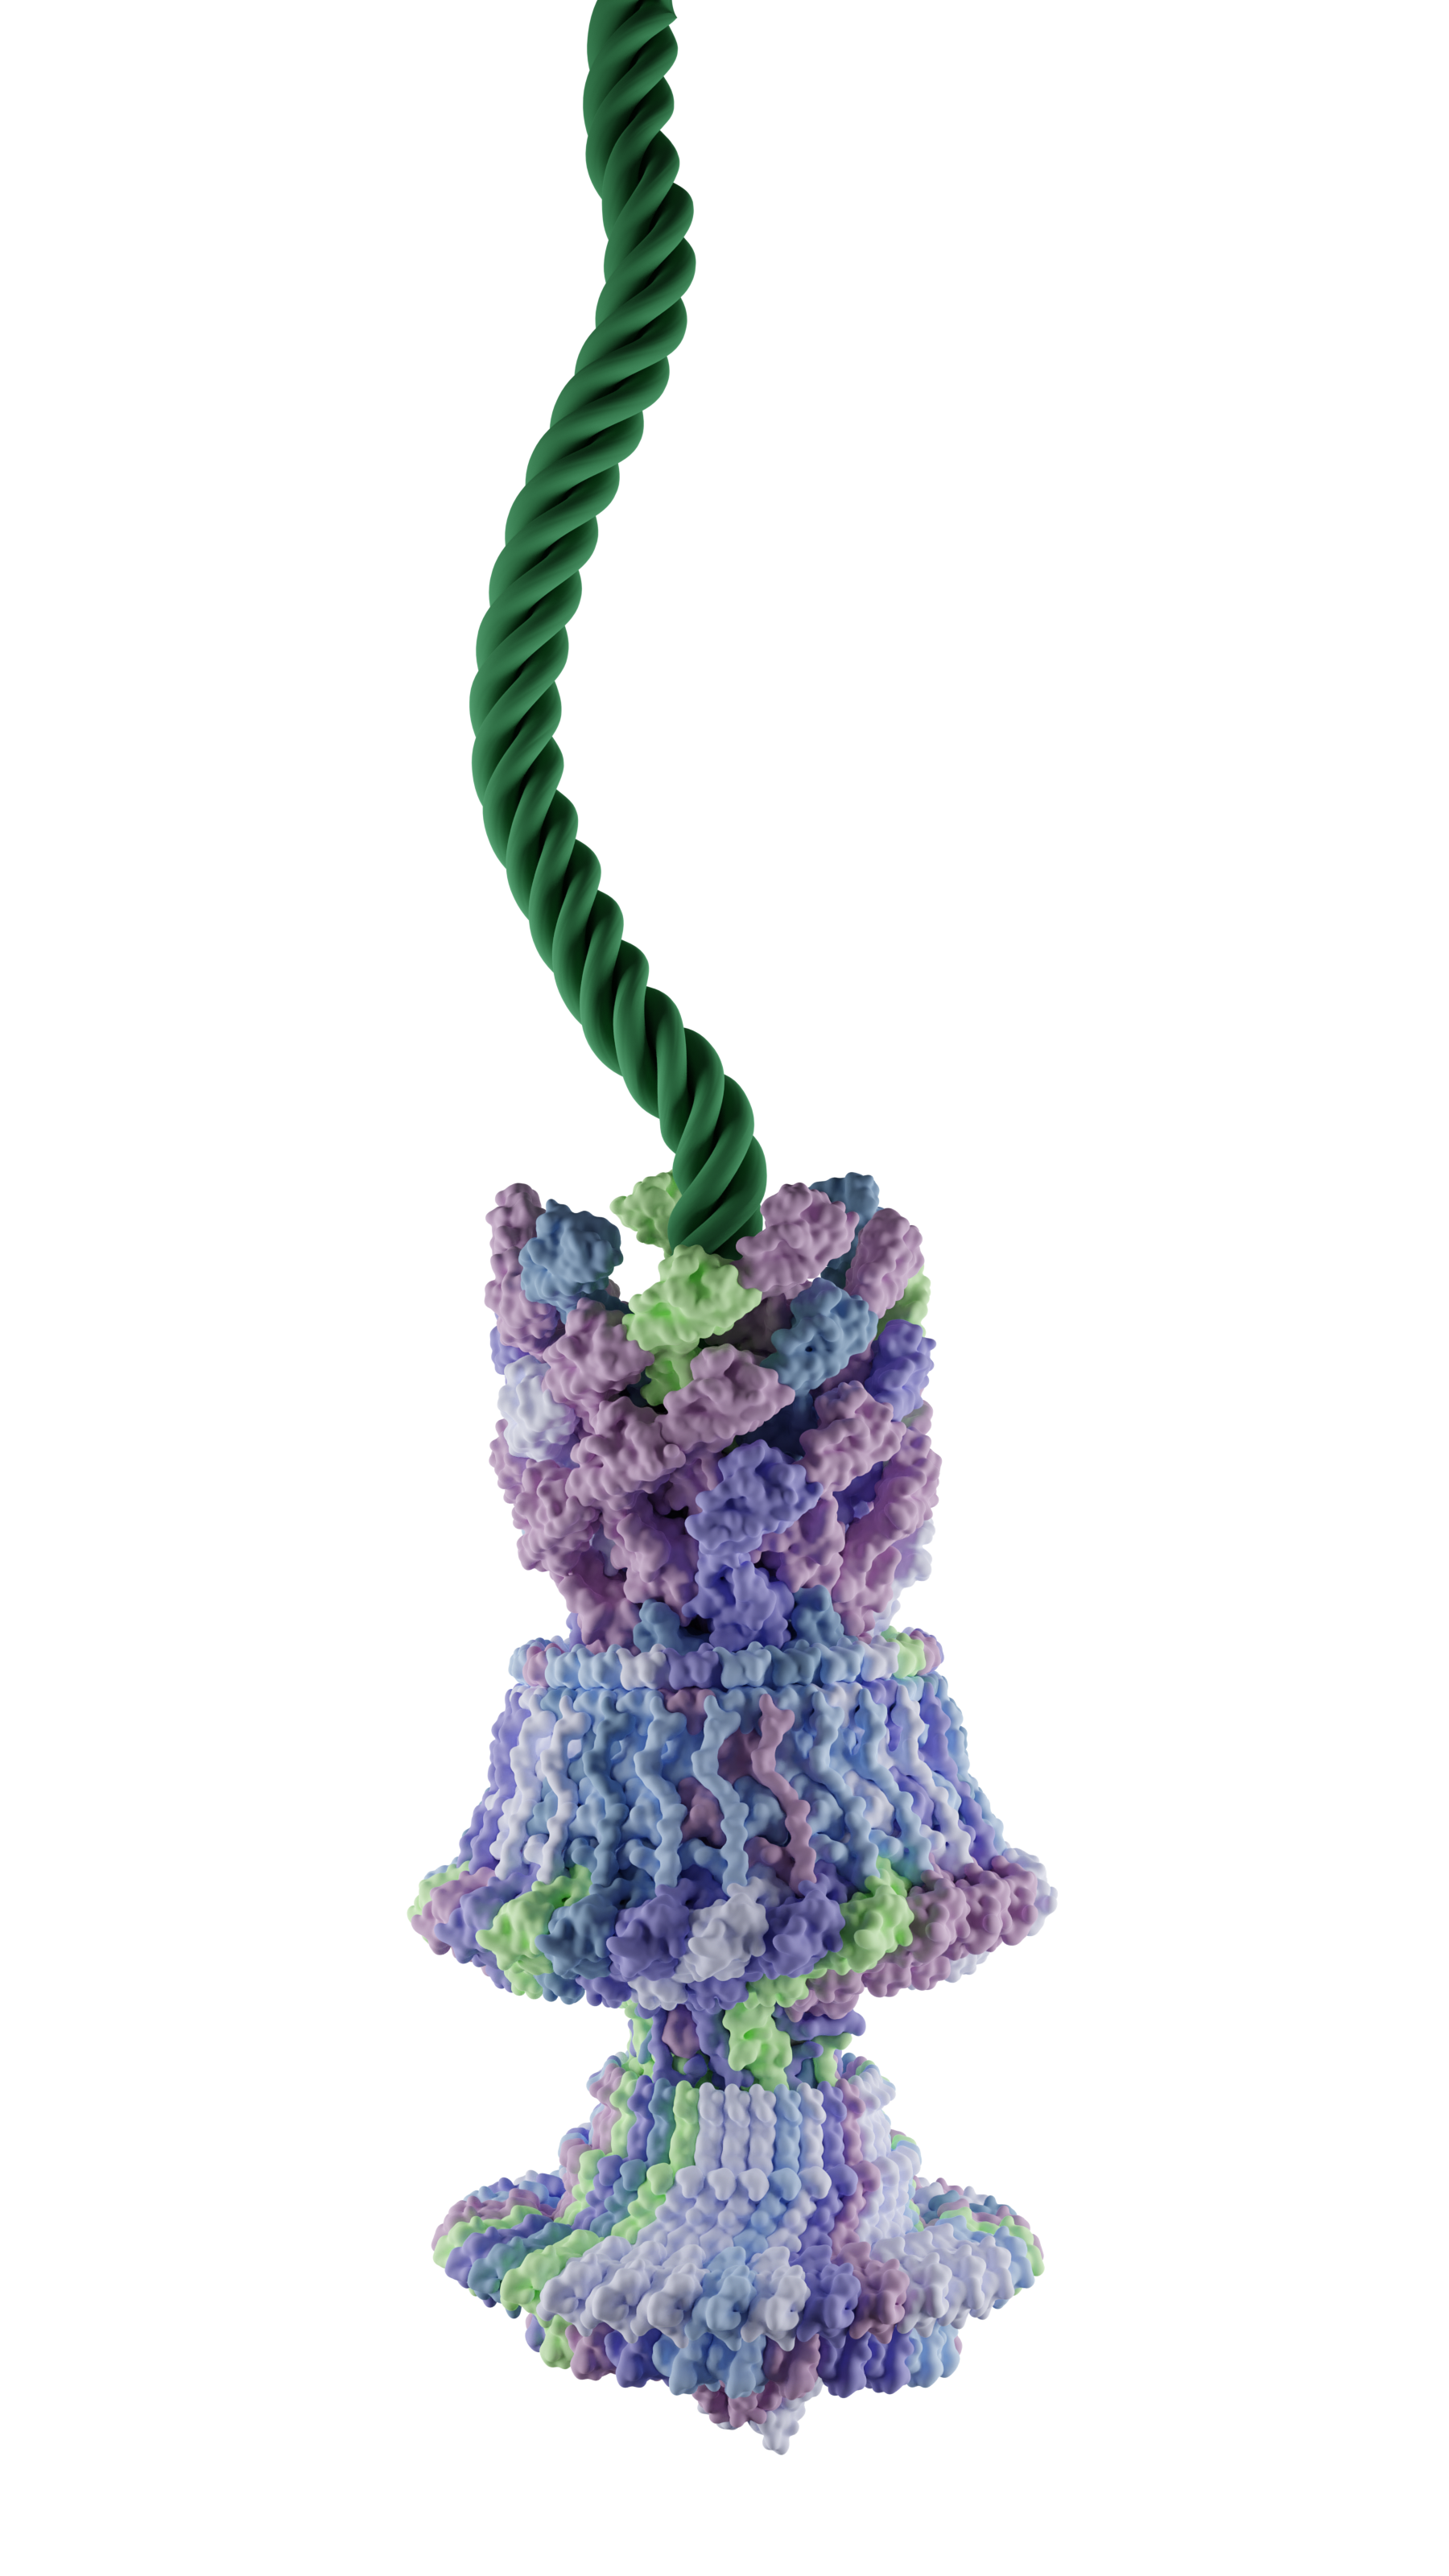
\includegraphics[width=0.80\textwidth]{Figures/flagella.png}
  \caption{write caption}
\end{center}
\end{figure}

\section{Biological Nanopores}

Biological nanopores are small perforations in a lipid bilayer membrane, created
by the central cylindrical cavity of a folded protein assembly. The majority of these
proteins are toxins produced by pathogenic bacteria. Their function in nature is to
perforate the membrane of a cell, causing the cell to depolarize, disrupting vital cell
functions. The perforation also induces an osmotic potential, causing cell nutrients to
spill into the environment. Both effects eventually result in the killing of the
cell.\cite{Peraro2016}

The reason scientists are interested in studying nanopores is related to their size.
These protein structures are generally only a few nanometres in diameter, making them
comparable in size to the tiny transistors found in modern computers. Retrieving
information form nano-scale processes has proven to be a challenging task. Developing
sensors to probe this small length scale is thereby very relevant. This is the exact task
nanopores provide a possible solution to, i.e. spectroscopy at the smallest
scale.

\subsection{Ionic Current Spectroscopy}

In recent years the study of nanopores became a popular research domain, mainly
due to the development of the nanopore-based ionic current spectroscopy. For the case of
biological nanopores, this method is depicted in Figure \ref{fig:IonicCurrentSpec}. A
reservoir, filled with a saline solution, is partitioned into two compartments by a
lipid bilayer. The membrane is perforated using a pore forming protein, for example
$\alpha$-Hemolysin.  When a potential difference is created over the membrane, the
nanopore mediates an ion current between the two liquid-filled compartments.

This ion current through the pore can accurately be measured. If the pore is empty we
refer to the measured current as the open-pore current. However, the applied electric
field also induces forces upon analytes dissolved in the liquid. The net result of these
interactions is a flux of analytes towards and in some cases through the nanopore.
Analytes located inside of the nanopore partially block the flow through the pore,
reducing the measured ion current. The time series of
these current fluctuations can be measured and identified with particular analytes in the
solution. These methods are so precise that they allow for single molecule
spectroscopy.\cite{Howorka2009}

The construction of the molecular machine discussed in this thesis is based on this
spectroscopy technique. Instead of studying analytes in the reservoirs, here
the configuration of a DNA thread trapped inside of the pore can be analysed using the
measured ion current.

It should be noted that besides these biological nanopores there are also inorganic
nanopores in development.\cite{Dekker2007} An example are solid state nanopores created
by making perforations in a semi-conductor wafer. Despite being currently not as
accessible as
biological nanopres, mainly due to their high production costs, this method has some
major advantages.  First of all the material properties provide a chemical robustness not
present in biological nanopores. Secondly, the production process also allows for easy
scalability
and customisability. While currently not as widely used as biological nanopores, solid
state nanopores will prove to be an important asset in the future of nanotechnology.

\begin{figure}[htpb!]
  \centering
  \includegraphics[width=0.72\linewidth, height=7.5cm]{Figures/IonicCurrentSpec2.png}
  \caption[Detailed illustration of ionic current spectroscopy.]{\linespread{0.1}
    {\linespread{0.1}\small  Illustration of the three primary scenarios encountered
      during ionic current
spectroscopy are depicted. Applying a potential difference over the membrane induces a
flow of cations (blue) and anions (red)
through the pore. If the pore is unobstructed, the mediated ion current is referred to
the open-pore current ($I_0$), shown in a). After a certain time $\Delta t_{d,1}$,
analyte $1$ approaches the pore entrance and partially blocks the pore current to the
current level $L_1$, as depicted in b). Due to the size of this analyte it is able to
translocate through the pore with a characteristic dwell time $t_{d,1}$. Both the
duration of translocation and the reduction in ion current depend on the
specific analyte properties . In c) a larger analyte is shown to block the pore current
to a lower level $L_2$. The larger size of this analyte forces it to exit back into the
cis-compartment with a characteristic dwell time $t_{d,2}$. Figure taken from reference
\cite{willems2021}.
}}
  \label{fig:IonicCurrentSpec}
\end{figure}




\subsection{$\alpha$-Hemolysin ($\alpha$-HL)}

The $\alpha$-Hemolysin ($\alpha$-HL) protein is the most commonly used pore forming
protein to create artificial nanopores. It is produced by Staphylococcus aureus, a
bacterium commonly found in the human skin microbiome.\cite{Bhakdi1991}

The $\alpha$-HL pore (PDBID\footnote{An identifier for entries in the Protein Data Bank
(PDB), a database for structural data of large biological
molecules.}:7AHL\cite{Song1859}) is an oligomeric complex
with multiple naturally occurring variations. The most typical configuration
is a heptameric structure, meaning that there are seven subunits, called protomers,
making up the pore complex.
The secondary structure elements consist principally of $\beta$-sheets \footnote{A
secondary protein structure created by hydrogen bonding between parallel or
antiparallel polypeptide strands forming extended $\beta$-pleated sheets.}, making
them a member of the $\beta$-barrel pore-forming toxins. Through both electrostatic and
hydrophobic interactions, the $\alpha$-HL is bound to the membrane of a target cell. Here
the monomers assemble to a 'prepore' complex that transitions to the stable pore complex
by inserting the $\beta$-barrel into the membrane.\cite{SUGAWARA2015226}

Structurally the shape of $\alpha$-HL resembles that of a hollow mushroom, see Figure
\ref{fig:alphaHL}. The total hight of the complex is $11\ nm$ and the maximum width is
measured to be $10\ nm$. The
internal chamber of the pore located at the cis-side of the membrane is called the lumen.
The lumen of $\alpha$-HL is quite constricted having a diameter of merely $3\ nm$.  At
the membrane the lumen chamber transitions into a protein stem, referred to as the
constriction of the pore. Here the diameter of the chamber is reduced to a minimum of
$1.5\ nm$. On the wall of $\alpha$-HL's inside chambers, the charges are relatively
uniformly distributed. \vspace{.4cm}

\begin{figure}[ht!]
  \begin{centering}
  \adjustbox{minipage=1.3em,valign=t}{\subcaption{}\label{sfig:testa}}%
  \begin{subfigure}[t]{\dimexpr.4\linewidth-1.3em\relax}
  \centering
  \includegraphics[width=\linewidth,valign=t]{Figures/ahl-front-c.png}
  \end{subfigure}%
  \adjustbox{minipage=1.3em,valign=t}{\subcaption{}\label{sfig:testc}}%
  \begin{subfigure}[t]{\dimexpr.4\linewidth-1.3em\relax}
  \centering
  \includegraphics[width=\linewidth,valign=t]{Figures/ahl-top-c.png}
  \end{subfigure}

  \vspace{1.cm}

  \adjustbox{minipage=1.3em,valign=t}{\subcaption{}\label{sfig:testd}}%
  \begin{subfigure}[t]{\dimexpr.4\linewidth-1.3em\relax}
  \centering
  \includegraphics[width=.7\linewidth,valign=t]{Figures/ahl-mon-c.png}
  \end{subfigure}
  \adjustbox{minipage=1.3em,valign=t}{\subcaption{}\label{sfig:testb}}%
  \begin{subfigure}[t]{\dimexpr.4\linewidth-1.3em\relax}
  \centering
  \includegraphics[width=\linewidth,valign=t]{Figures/ahl-elec.png}
  \end{subfigure}%


  \caption[Structural overview of the $\alpha$-Hemolysin ($\alpha$-HL) pore forming
  protein.]{\linespread{0.816}{\small (a) Side view and (b) top view of the
  heptameric $\alpha$-hemolysin ($\alpha$-HL) protein structure. The mushroom shape
  arising from the protomer assembly is clearly shown. (c) Protomer subunit from the
  pore complex, where the two antiparallel $\beta$ strands composing the $\beta$ barrel
  are visible. (d) Estimation of the charge distribution on the cross-section of
  the merged density surface of $\alpha$-HL. All images were rendered using
  ChimeraX. \cite{ChimeraX, Song1859}}}
  \label{fig:alphaHL}

  \end{centering}
\end{figure}

\begin{figure}[ht!]
  \begin{centering}
  \adjustbox{minipage=1.3em,valign=t}{\subcaption{}\label{sfig:testa}}%
  \begin{subfigure}[t]{\dimexpr.3\linewidth-1.3em\relax}
  \centering
  \includegraphics[width=\linewidth,valign=t]{Figures/clya-front-c.png}
  \end{subfigure}%
  \adjustbox{minipage=1.3em,valign=t}{\subcaption{}\label{sfig:testb}}%
  \begin{subfigure}[t]{\dimexpr.35\linewidth-1.3em\relax}
  \centering
  \includegraphics[width=\linewidth,valign=t]{Figures/clya-top-c.png}
  \end{subfigure}

  \vspace{1.cm}

  \adjustbox{minipage=1.3em,valign=t}{\subcaption{}\label{sfig:testb}}%
  \begin{subfigure}[t]{\dimexpr.35\linewidth-1.3em\relax}
  \centering
  \includegraphics[width=.35\linewidth,valign=t]{Figures/clya-mon-c.png}
  \end{subfigure}%
  \adjustbox{minipage=1.3em,valign=t}{\subcaption{}\label{sfig:testa}}%
  \begin{subfigure}[t]{\dimexpr.3\linewidth-1.3em\relax}
  \centering
  \includegraphics[width=\linewidth,valign=t]{Figures/clya-elec.png}
  \end{subfigure}%

  \caption[Structural overview of the Cytolysin A (ClyA) pore forming
  protein.]{\linespread{0.816}{\small (a) Side view and (b) top view of the
  dodecameric Cytolysin A (ClyA) protein structure. The cylindrical shape
  arising from the protomer assembly is clearly shown. (c) Protomer subunit from the
  pore complex, where the $\alpha$-tongue is visible. (d) Estimation of the charge
  distribution on the cross-section of the merged density surface of ClyA. All images
  were rendered using ChimeraX. \cite{ChimeraX, Peng2019}}}
  \label{fig:ClyA}

  \end{centering}
\end{figure}

\subsection{Cytolysin A (ClyA)}

The Cytolysin A (ClyA) is a larger type of pore forming protein first found to be
secreted by Escherichia coli strains. \cite{Mueller2009} The larger size of its lumen
allows for
different applications compared to smaller complexes like $\alpha$-HL. The
larger diameter of the pore's stem allows for translocation of double stranded DNA, as
demonstrated in the molecular machine discussed in this thesis.

The ClyA pore (PDBID:6MRT\cite{Peng2019}) is an oligomeric complex most typically found
in a dodecameric configuration,  meaning that there are twelve subunits, called
protomers, making up the pore complex. In nature small variations on this configuration
are found.
% \begin{wrapfigure}[38]{l}{0.19\textwidth}
%   \begin{center}
%     \includegraphics[width=0.2\textwidth]{Figures/DNAStrand.png}
%   \end{center}
%   \caption{\linespread{0.816}{\small An illustration of the double helical structure of
% DNA. Shown is the BDNA form rendered using PDB data and Blender.}}
% \end{wrapfigure}
The secondary structure elements consist principally of
$\alpha$-helices\footnote{A secondary protein structure created by stabilising a coiled
peptide chain with hydrogen bonds, forming a right handed-helix configuration.},
making it a member of the $ \alpha$-pore-forming toxins. The protein formation is induced
by the hydrophobic interactions between the monomers $\beta$-hairpin and the solvent. The
main structural rearrangement in this process consists of swinging out this hairpin and
inserting the resulting $\alpha$-tongue into the membrane. After this transition, the
membrane-bounded monomers oligomerize to form the final pore structure.\cite{Benke2015}

Structurally the shape of ClyA resembles that of two hollow cylinders stacked on top of
each other, see Figure \ref{fig:ClyA}. This cylinder approximation will be important
later on in this thesis, where
it will be used to create a simplified model of the nanopore. The total hight of the
complex is $14\ nm$ and the maximum width is measured to be $11\ nm$. The lumen's size of
this
nanopore differentiates it from the previously discussed $\alpha$-HL. The cis-entrance of
the lumen measures $6\ nm$, while the constricted side of the pore is still $3.6\ nm$ in
diameter.  In contrary to the $\alpha$-HL, the inside surface of ClyA has a net negative
charge, promoting the capturing of positive ions. On the contrary, this excess charge
will induce a significant Coulomb repulsion between the pore and negatively charged
analytes.


\section{Deoxyribonucleic acid (DNA)}

\begin{wrapfigure}{r}{0.23\textwidth}
  \begin{center}
    \includegraphics[width=0.20\textwidth]{Figures/DNA1.png}
  \end{center}
  \caption{caption nog maken}
\end{wrapfigure}

Deoxyribonucleic acid (DNA) is a long biopolymer composed of two strands, commonly found
in its characteristic double helical structure. DNA is most famously know for storing the
genetic code in each of our cells. The existence of this genetic code was already
postulated by the Greek philosopher Aristotle. He developed a heredity theory based
upon "blueprints" in which he tried to explain why physical traits where passed on from
generation to generation. This theory would go unnoticed until in 1869
Friedrich Meicher discovered a new microscopic substance found on discarded
surgical bandages. He would call this substance "Nuclein" since it originated
form the nucleus of the cell. Later it was found that this new substance, now called
"Deoxyribonucleic acid" or DNA, serves as a blueprints in our modern theory of
heredity.

The structure of DNA was first determined by Rosalind Franklin using X-ray
crystallography. Their research concluded that DNA consists of
two individual strands coiled around each other in a double helical structure. Each
strand is a chain of monomers, which we call nucleotides. A nucleotide is made up of a
deoxyribose sugar, phosphate group and one of four nitrogenous bases: cytosine(C),
guanine(G), adenine(A) or thymine(T). The covalent bonds that give both strands structure
are formed between consecutive phosphate groups, together they make up the backbone of
the strand. To form the double helix, two backbones are held together by
selective hydrogen bonds occurring between corresponding bases of opposing strands. These
dipole interactions give rise to a selection rule, forming only A-T and C-G pairs.

Since the binding of the two strands is mediated by hydrogen bonding, the association an
dissociation is possible. The study of these processed is called DNA thermodynamics. The
dissociation process of double stranded DNA (dsDNA) is called DNA melting, resulting in
two individual strands of single stranded DNA (ssDNA). The reverse process is called DNA
hybridisation, which is the selective binding of complementary nucleotides to form dsDNA.

The double helix structure of DNA comes in three different types, B-DNA, A-DNA and Z-DNA,
all having a slightly different geometric arrangement. In nature the B-form is most
commonly observed, it is characterised by a right-handed helix and the coplanarity
between the complementary bases as shown in Fig. ... . A helical twist of B-DNA consists
of around 10 bp's having a net helical pitch of 0.34nm. During this thesis when analysing
DNA we refer to the B-DNA form.

When Studying DNA the statistical theory polymer physics is a usefull tool. A atomistic
resolution is not needed to accuratly descibe process involving longer length scales.
Reducing the complexity of the DNA to the monomers level is often justified, allowing us
to use more general results of polymer physics.



\section{Polymer Physics}
The theory of polymer physics logically starts with defining the notion of a polymer, for
simplicity we will limit the discusison to linear polymers. The building blocks of a
polymer are called monomers, linked together to from a chain. The configuration of this
chain is determined by the position vectors of each monomers, ${\boldsymbol{r}_0,
\boldsymbol{r}_1, \dots, \boldsymbol{r}_N}$. Each pair of consecutive monomers is linked
together, giving rise to the bond vectors u_i = ... During this discussion we will assume
these bonds to be inextensable, i.e. a fixed segment length $|\boldsymbol{u}_i| = a$.

$\boldsymbol{u}_i = \boldsymbol{r}_i - \boldsymbol{r}_{i-1}$

The Kratky-porod model is an example of a mathermatically simple
model that results in a suprisingly realistic description of a polymer.

\begin{equation}
    E_{WLC}= -\kappa \sum_{i=1}^{N-1} \boldsymbol{\hat{u}_i} \cdot \boldsymbol{\hat{u}}_{i+1}
    = -\kappa
    \sum_{i=1}^{N-1} \cos\theta_i,
\end{equation}

\begin{equation}
\begin{aligned}
    \label{210}
    Z_{\mathrm{WLC}}(N, T)
    &= \left[\int_{0}^{\pi} d \theta \sin \theta e^{\beta \kappa \cos \theta}\right]^{N}
\end{aligned}
\end{equation}

\begin{equation}
    Z_{\mathrm{WLC}}(1, T)=\int_{0}^{\pi} d \theta e^{\beta \kappa \theta}=\frac{2 \sinh(\beta
    \kappa)}{\beta \kappa}
\end{equation}
Using the relation:
\begin{equation}
    \left\langle\cos \theta_{i+1}\right\rangle
    =\frac{\partial \log Z_{\mathrm{WLC}}(1, T)}{\beta \partial \kappa},
\end{equation}
one can calculate the mean dot product between two consecutive bonds:
\begin{equation}
    \left\langle\boldsymbol{u}_{i} \cdot \boldsymbol{u}_{i+1}\right\rangle
    = \left\langle\cos \theta_{i+1}\right\rangle
    = \frac{1}{\tanh(\beta \kappa)} - \frac{1}{\beta \kappa}.
\end{equation}
Which in the limit of $\beta \kappa \gg 1$ leads to:
\begin{equation}
    \langle\cos \theta\rangle \approx 1-\frac{1}{\beta \kappa}.
\end{equation}
This condition is true for low temperatures or large stiffness between neighbouring bonds (large \kappa). In the following equations the persistence length $l_b$ is mathematically introduced:
\begin{equation}
\begin{aligned}
    \left\langle\boldsymbol{u}_{1} \cdot \boldsymbol{u}_{n+1}\right\rangle
    &=\left\langle\boldsymbol{u}_{1} \cdot \boldsymbol{u}_{n}\right\rangle\left\langle\cos
    \theta_{n}\right\rangle
    &= a^{2}\langle\cos \theta\rangle^{n}
    &=a^{2} \exp \bigg{[} -\frac{n a}{l_{b}} \bigg{]},
\end{aligned}
\end{equation}
where $l_b \equiv \frac{a \kappa}{k_{b} T}$ and $a$ is the constant bond length for the discrete WLC model.

The bending persistence length $l_b$ can be related to the end-to-end boldsymboltor $\boldsymbol{R}$ in
the continuum limit. For example can be rewritten using the arc-length parameter $s$
where $0 \leq s \leq L$ and $L = Na$ as:
\begin{equation}
    \label{hoi}
    \langle\widehat{u}(q) \cdot \widehat{u}(q+s)\rangle= e^{-s / l_{\mathrm{p}}}.
\end{equation}
The continuum version of the end-to-end boldsymboltor is:
\begin{equation}
    \boldsymbol{R}=\int_{0}^{L} \widehat{u}(s) d s.
\end{equation}
Taking the square of this expression and averaging over it, we obtain the following:
\begin{equation}
\begin{aligned}
    \left\langle\boldsymbol{R}^{2}\right\rangle
    &= \int_{0}^{L} d s d s^{\prime}\left\langle\widehat{u}(s) \cdot
  \widehat{t}\left(s^{\prime}\right)\right\rangle \\
    &= 2 l_{\mathrm{b}} L\left\{1-\frac{l_{\mathrm{b}}}{L}\left(1-e^{-L /
l_{\mathrm{b}}}\right)\right\}.
\end{aligned}
\end{equation}

Explain here two limiting cases of above expression. This leads to a interpretation of
what the persistence length means intuitively. -> length over which the correlations
between bond boldsymboltors are lost.

\newpage
\section{Computer Simulations}

The theory of classical mechanics is often regarded as the first major breakthrough in
the field of physics. For every aspiring physicist this is still the starting point of
their studies. Unfortunately, getting to know these relatively simple laws of nature,
leads to the inescapable realisation that these theories are expressed in mathematical
formalisms that are only analytically solvable in few idealised scenarios. Applying these
formulas to a problem consisting of just more then two particles already leads to
practically unsolvable equations.\\

Although it is often times not possible to find an exact solution to equations
related to complex physical systems, finding reasonable approximations to their solution
is achievable. One popular method to analyse the dynamics of complex systems is the use
of simulations.\\

\begin{wrapfigure}{r}{0.5\textwidth}
  \begin{center}
    \includegraphics[width=0.38\textwidth]{Figures/WaterModel.png}
  \end{center}
  \caption{Example of an expanded model of a simple liquid (J L Finney, Ph.D thesis)}
\end{wrapfigure}

Simulations have a rich history within physics and engineering, starting even before the
invention of the computer.

An example of one of these mechanical simulations is the Waterloopkundig Laboratorium
or
currently the waterloopbos, a scale model of important
Dutch waterways, where the influence of waves on harbours and docks was studied. This
simulation provided revolutionary insights into the behaviour of water and played an
important part in the design of the famous Delta Works.\\

Another more relevant example is the use of mechanical simulations to study the
structure of water.  In the early 20th century physicist J.D. Bernal and his fellow
researchers build various ball and stick models of water to analyse the possible 3D
configurations of water molecules in a liquid. Their research eventually explained the
peculiar physical properties of water from a atomistic perspective. However useful these
mechanical simulations turned out to be, the biggest drawback of the method was the
extreme cost of labour involved with their construct. As Bernal alluded to in his
famous 1962 lecture,

\begin{quote}
\dots I took a number of rubber balls and stuck them together with rods of a
selection of different lengths ranging from 2.75 to 4 inch. I tried to do this in the
first place as casually as possible, working in my own office being interrupted every
five minutes or so and not remembering what I had done before the interruption.\dots
\end{quote}

After the first computer simulations where performed in the Los Alamos labs, the
popularity of simulations rapidly increased. The remarkable explanatory power of
simulations, combined with the relative easy construction of computer models, lead to a
fast adoption of computer simulations in the scientific community. Within the context of
this thesis, computer simulations are used to study the mechanics of
the DNA polymer. Due to the high number of atoms in a typical system, it is generally
not possible to find an analytical solution to their equations of motion. In this
context, simulations are often used to gain an insight into the complex dynamics of the
system and guide the developments of more simple approximate theories. The simulations
act as a bridge between the microscopic constituents of the systems and the macroscopic
properties we want to understand.


\subsection{Molecular Dynamics Simulations}
Molecular Dynamics (MD) is a computer simulation technique, used to analyse
the dynamics of a classical many-body system. The central idea of this method is to
generate all the trajectories in a system of $N$ particles by numerically
integrating the classical equations of motion,
\[
m_i \frac{d^2 \boldsymbol{r_i}}{dt^2} = \boldsymbol{f_i}, \quad \boldsymbol{f_i} = -
    \frac{\partial}{\partial \boldsymbol{r_i}} \mathcal{U}_i, \quad for\ i \in N.
\]
The motion of the particles are governed by the forces $f_i$ acting upon them, which are
usually derived from the interaction potentials $U_i$.
Solving these differential equations is achieved by employing a discretized time
integration scheme.  Algorithm 1 shows the typical structure of a molecular dynamics
simulation. The discretization resolution is conventionally called the time step of the
simulations denoted by $\Delta t$.\\

\noindent There are a large number of different integrations schemes that one can choose
from, where the choice depends entirely on the system at hand.
When working with an isolated system -- i.e. microcanonical ensemble --, logically an
energy conserving integrator is needed. The canonical
choice for this type of integration scheme is the Velocity-Verlet algorithm. This
algorithm is an example of leapfrog integration, where the updating of the positions
and velocities are interleaved at different points in time. The major strength of this
type of algorithm is that it turns out to be a symplectic integrator, which means the
errors on the conserved energy are bounded.

On the other hand, when a system is in contact with a thermal reservoir --i.e. canonical
ensemble-- not the total energy is conserved, but rather the temperature of the
simulation is fixed. To achieve this, a thermostat is implemented in the MD
simulation. A typical thermostat attempts to negate any drift in temperature by
appropriately importing or exporting energy to the system after each timestep.
Poplular examples of thermostats are the Nos\'e-Hoover thermostat or the Langevin
thermostat.  The latter regulates the temperature by introducing an implicit solvent to
the simulation that gives rise to random thermal kicks. The resulting equations of motion
are the Langevin equations given by,

\begin{equation}
    m_i \frac{d^2 \boldsymbol{r}_i}{dt^2} = - \nabla \mathcal{U}_i - \gamma_i \frac{d
    \boldsymbol{r}_i}{d t} +
    \xi_i(t),
\end{equation}
where $\gamma_i$ is known  as the friction coefficient and $\xi_i(t)$ a random force
acting upon the particles. The combination of the last two terms fully capture the
statistical consequences of the solvent interacting with the system.


\begin{algorithm}
    \SetKwFunction{isOddNumber}{isOddNumber}
    \SetKwInOut{KwIn}{Input}

    \KwIn{Configuration of the system at $t=0$}

    $newList = [\ ]$

    \tcc{For odd elements in the list, we add 1, and for even elements, we add 2.}

    \For{$i \leftarrow 0$ \KwTo $n-1$}{
        \eIf{$\isOddNumber(a_i)$}{

            $newList.append(a_i + 1)$ \tcp*[f]{Some thought-provoking comment.}
         }{
            \tcp{Another comment}
            $newList.append(a_i + 2)$
         }
    }

    \KwRet{$newList$}
    \caption{The Velocity Verlet algorithm}
\end{algorithm}

% \begin{center}
% 	\begin{tikzpicture}[
% 	squarednode/.style={rectangle, draw=blue!60, fill=blue!5, very thick, minimum width=50mm,
% 	minimum height=5mm},]
% 	%Nodes
% 	\node[squarednode]      (step1)                        {1};
% 	\node[squarednode]      (step2)       [below= 3mm of step1] {2};
% 	\node[squarednode]      (step3)       [below= 3mm of step2] {3};
% 	\node[squarednode]      (step4)       [below= 3mm of step3] {4};
% 	\node[squarednode]      (step5)       [below= 3mm of step4] {5};
% 	\node[squarednode]      (step6)       [below= 3mm of step5] {6};
% 	\node[squarednode]      (step7)       [below= 3mm of step6] {7};
% 	\node[squarednode]      (step8)       [below= 3mm of step7] {8};
%
% 	%Lines
%     \draw[very thick, ->] (step1.south) -- (step2.north);
% 	\draw[very thick, ->] (step2.south) -- (step3.north);
% 	\draw[very thick, ->] (step3.south) -- (step4.north);
% 	\draw[very thick, ->] (step4.south) -- (step5.north);
%     \draw[very thick, ->] (step5.south) -- (step6.north);
% 	\draw[very thick, ->] (step6.south) -- (step7.north);
% 	\draw[very thick, ->] (step7.south) -- (step8.north);
% 	\draw[very thick, ->] (step8.west)  -- +(-0.4,0) |-(step2.west);
% 	\end{tikzpicture}
% \end{center}

\subsection{Coarse Grained modelling}
As most thing do, molecular dynamics simulations have their pitfalls. A commonly
encountered problem is the rapidly increasing computational cost, when the number of
particles in the system increase. If not addressed, this would limit the scope of MD
simulations to systems of a few particles over short time-scales.\\

During these simulations the most costly calculations involve the non-bonded
interactions in the system. These interatomic interactions make the computational
complexity for rudimentary MD simulations scale as $O(N^2t)$, where $N$ is the number of
particles in the system and $t$ the simulation time. This bad scaling behaviour comes
from the fact, that for each individual particle all the other particles are contributing
to its interaction potential. To improve this scaling behaviour, the non-bonded
interactions in a MD simulation are almost always truncated. This localization of the
interatomic interactions has the nice effect that not all atoms are involved in every
calculation. Efficient algorithms, like the multigrid method, have been derived to
improve the scaling complexity of MD simulations up to $O(Nt)$.\\

Coarse graining is a method to further optimize molecular dynamics simulations.
In contrary to all atom simulations, where each atom is explicitly represented in the
simulation, in coarse grained simulations multiple atoms are grouped together to form
generalised pseudo-atoms with their respective pseudo-interaction.

There are two distinctly different ways to construct a coarse grained model. The first
method starts from the all atom model of the system and generalises nearby atoms into
larger pseudo-atoms, this is called the bottom up approach. The second method focuses
more on the precise reproduction of experimental results, rather than
the precise small scale dynamics. Here larger pseudo-atoms are designed, based upon
characteristic patterns in the structure, after which the pseudo-interactions are tweaked
to accurately reproduce the system's dynamics.

In the case of DNA simulations, coarse graining turned out to be a very important method.
Previous all atom simulations of DNA polymers were restricted to simulations of less then
hundred baisepairs over only a few microseconds. Studying large scale systems, often
encountered in DNA technology, was only possible after the development of coarse grained
models. A few examples of commonly used coarse grained models of DNA are Martini, 3SPN
and oxDNA.

\begin{figure}[htpb]
    \centering
    \includegraphics[width=0.6\linewidth]{Figures/CoarseGrained.png}
    \caption{zelf nog maken}%
    \label{fig:Figures/CoarseGrained}
\end{figure}


\cleardoublepage
% \vspace{-1cm}
% \epigraph{Given for one instant an intelligence which could comprehend all
% the forces by which nature is animated and the respective positions
% of the beings which compose it, if moreover this intelligence were vast
% enough to submit these data to analysis, it would embrace in the same
% formula both the movements of the largest bodies in the universe and
% those of the lightest atom; to it nothing would be uncertain, and the
% future as the past would be present to its eyes.}
% {--- \textup{Pierre-Simon Laplace}}
\chapter{The DNA Nanopiston}
Duidelijk duiden dat dit hoofdstuk gebaseerd is op de paper van stefanos en bajoumi.
\section{Rotaxane Formation}



\begin{figure}[ht]
  \begin{centering}
  \adjustbox{minipage=1.3em,valign=t}{\subcaption{}\label{sfig:testa}}%
  \begin{subfigure}[t]{\dimexpr.5\linewidth-1.3em\relax}
  \centering
  \includegraphics[width=.9\linewidth,valign=t]{Figures/RConstruction1.png}
  \end{subfigure}%
  \vspace{1cm}
  \adjustbox{minipage=1.3em,valign=t}{\subcaption{}\label{sfig:testa}}%
  \begin{subfigure}[t]{\dimexpr.5\linewidth-1.3em\relax}
  \centering
  \includegraphics[width=.9\linewidth,valign=t]{Figures/RConstruction2.png}
  \end{subfigure}%
  \vspace{1cm}
  \adjustbox{minipage=1.3em,valign=t}{\subcaption{}\label{sfig:testb}}%
  \begin{subfigure}[t]{\dimexpr.5\linewidth-1.3em\relax}
  \centering
  \includegraphics[width=.9\linewidth,valign=t]{Figures/RConstruction3.png}
  \end{subfigure}
  \caption{This is a figure}
  \label{fig:test}
  \end{centering}
\end{figure}

\section{Operating principles}

Having successfully constructed the DNA nanopiston, now the operation cycle can be
discussed. For convenience, we take the rotaxane-ds configuration as the starting point
of this cycle. The power stroke of the molecular machine is initiated by bringing the
appropriate chemical fuel, ssDNA $4$ $(0.5\ \mu M)$, into solution at the trans-side. The
DNA strand is fully complementary to ssDNA $2$, thereby inducing a toehold-mediated
strand displacement. Here the flexible overhang located at the end of ssDNA $2$, referred
to as the toehold, is used to mediate the hybridisation of ssDNA $2$ and $4$ (Fig ..).

During the strand displacement reaction, two possible transient states can possibly
occur. On of the possibly scenario's describes the hybridisation happening inside of the
nanopore. This scenario is deemed to be unlikely, since this process would require three
strands of ssDNA to be simultaneously present inside the constriction of the nanopore.
Alternatively, the hybridisation can take place outside of the nanopore, in the
trans-side of the reservoir. This process implies that the neutravidin protein would
enter the lumen of the pore, which has been showed by previous studies to be possible.
This second scenario is thereby thought of as the most probable.

The resulting configuration is called the rotaxane-ss in view of the fact that it is
predominately composed of ssDNA. During this process a DNA duplex, composed of the ssDNA
2 and 4, is released into the trans-side of the reservoir.

The following step in the cycle consists of the piston's recovery stroke, induced by
bringing $0.5\ \mu M$ of ssDNA $2$ into solution at the cis-side. The strand hybridises
with the rotaxane-ss forming the rotaxane-ds structure and completing the cycle.
Each piston interaction transports one cargo strand, ssDNA $2$, from the cis- to the
trans-side of the nanopore, turning over one fuel strand in the process.


Important to note is that no external potential is specified for operating the DNA
nanopiston. In contrast to earlier DNA transporters, the piston is able to function in a
range of applied transmembrane biases. Experimentally it is verified that the
cycle operates at positive, $+20\ mV$, $+50\ mV$ and $+100\ mV$ and negative, $−20\ mV$.
The main factor determining the operational limits for a negative bias is most likely
the inability of the fuel strand to hybridise with the toehold of rotaxane-ds. The
ineptitude of the cargo to bind to the toehold is an overall limiting factor in the
operation process, resulting in faster cycles at positive then at negative applied bias
(Fig ...).

The ability of the nanopiston to transport cargo both with and against an external bias
is an important property of the molecular machine. The entropic interactions between the
DNA strands and the nanopore are expected to play an important role in this behaviour.
The piston operating at a wide range of positive biases for most likely results from the
entropic interactions between the toehold and the constricted pore entrance.  Since the
toehold is composed of flexible ssDNA is kept out the condiment of the trans-entrance to
the pore making it available for the toehold displacement reaction to happen.
After the rotaxane-ss is formed , the neutravidin protein is most likely found in the
lumen of the nanopore. The entropic interaction force resulting from the highly confined
ssDNA strand aids the rotaxane-ss to push the neutravidin bead into the cis-compartment
of the reservoir, making the hybridisation reaction possible to recover the initial
rotaxane-ds configuration.

Shows the limitation of the experimental analysis of the pore, only view into the system
is thought the measured current. To get a more in-depth understanding of the conformal
fluctuations of the pore  computation analysis was performed in the form of molecular
dynamics simulations.


% Figure 2.2a shows the measured current over through the nanopore during the operation
% cycle. The ionic current of rotaxane-ss is lower than the blocked current ofrotaxane-ds
% most likely reflecting the coiled structure of ssDNA inside the nanopore. Shows the
% limitation of the experimental analysis of the pore, only view into the system is
% throught the measured current. To get a more in-depth understanding of the conformal
% fluctuations of the pore computation analysis was performed in the form of molecular
% dynamics simulations.


%  ⡏⢱ ⠄ ⣰⡀   ⣀⡀ ⢀⡀ ⢀⡀   ⢀⡀ ⡀⣀ ⢀⡀ ⢀⡀ ⣀⡀ ⢀⣀   ⣇⡀ ⠄ ⠠   ⢀⣀ ⢀⣀ ⣇⡀ ⡀⣀ ⠄ ⠠ ⡀⢀ ⢀⡀ ⣀⡀
%  ⠧⠜ ⠇ ⠘⠤   ⠇⠸ ⠣⠜ ⣑⡺   ⠣⠭ ⠏  ⣑⡺ ⠣⠭ ⠇⠸ ⠭⠕   ⠧⠜ ⠇ ⡸   ⠭⠕ ⠣⠤ ⠇⠸ ⠏  ⠇ ⡸ ⠱⠃ ⠣⠭ ⠇⠸
% -----------------------------------------------------------------------------------------

% misschien bij de biological nanopores.
% Electrophoretic, electro-osmotic and entropic forces are, in principle, acting on the
% rotaxanes. The electrophoretic force sets the negatively charged DNA in motion, under the
% action of the applied bias (from cis to trans for
% ∆?? > 0 ). Electroosmosis generates an opposing force, arising from the motion of cations
% accumulated on the walls of the negatively charged ClyA pore and the DNA thread. Finally,
% the entropic force is solely geometry specific, and pushes the rotaxane towards
% conformations with high configurational entropy. Entropic forces are expected to play an
% important role in the rotaxanes studied here, which are composed of stiff dsDNA and
% flexible ssDNA parts.



\begin{figure}[ht]
  \begin{centering}
  \adjustbox{minipage=1.3em,valign=t}{\subcaption{}\label{sfig:testa}}%
  \begin{subfigure}[t]{\dimexpr.95\linewidth-1.3em\relax}
  \centering
  \includegraphics[width=\linewidth,valign=t]{Figures/FluctuationRotaxane.png}
  \end{subfigure}%
  \vspace{0.5cm}
  \adjustbox{minipage=1.3em,valign=t}{\subcaption{}\label{sfig:testb}}%
  \begin{subfigure}[t]{\dimexpr.5\linewidth-1.3em\relax}
  \centering
  \includegraphics[width=\linewidth,valign=t]{Figures/RotaxaneCycle.png}
  \end{subfigure}
  \caption{This is a figure}
  \label{fig:test}
  \end{centering}
\end{figure}

\section{Coarse-grained simulations}

During the discussion of the nanopiston's operation cycle it was hypothesised
that entropic interactions play an important role in its functioning. Studying these
phenomena is experimentally rather difficult, since all results are inferred based upon
the measured current traces and known interactions between the different elements of the
system. To obtain a more in-depth understanding of these interactions, computer
simulations are needed to proved the necessary insights.

In view of these challenges, a coarse-grained model of the DNA nanopiston was devised by
Bayoumi et al. The model is used to perform molecular dynamics simulations of  the
conformational fluctuations of the rotaxane at zero bias. Performing the simulations was
done by using the Large-scale Atomic/Molecular Massively Parallel Simulator (LAMMPS) and
its implementation of a Langevin intergrator.[.]

The coarse-grained model is composed of four types of interacting pseudo
atoms, all taking into account excluded volume interactions via repulsive Lennard-Jones
potentials. First of all, the Clya nanopore is represented by three vertically stacked
open cylinders, with diameters 6 nm, 5.5 nm and 2.9 nm from the cis- to the trans-side.
To take into account the electrostatic DNA-nanopore interactionsthe, the cylinder radii
are appropriately adjusted from the pore's geometry reported in.[.]
These electrostatic interactions predominately arise from excess negative charge in the
constriction of ClyA, resulting in a reduced size of the trans-cylinder. Note that the
pore is excluded from the Langevin integration, resulting in a static pore model.

A semiflexible bead-and-spring model is used to simulate the rotaxane. Each spherical
bead represents one ssDNA nucleotide or five dsDNA base pairs, respectively having a
diameter of $1\ nm$ and  $2.2\ nm$. The bond connecting each consecutive pair of beads is
represented by a harmonic spring. Determining the bond stiffness is done by means of the
equipartition theorem, from which we find
  \begin{equation}
    k_{bond} = \frac{3 k_b T }{ \langle a \rangle},
  \end{equation}
here $\langle a \rangle$ is the equilibrium bond length taken to be $0.68\ nm$ or $1.7\
nm$ for ssDNA and dsDNA respectively. In this model the bending rigidity of the DNA
polymer is taken into account. This effect is modelled as previous seen in the discrete
worm like chain, where the angle between consecutive bond vectors is assigned a harmonic
potential. Using Equation .., the bending rigidity is determined by
  \begin{equation}
    \kappa_{bend} = \frac{l_{p} \kappa_b T}{\langle a \rangle},
  \end{equation}
  where $l_p$ is the persistence length of the ssDNA ($2.2\ nm$) and dsDNA ($45\ nm$)
strands. The difference in persistence length results in the relatively large flexibility
of ssDNA strands.

The last components of the coarse-grained model are the neutravidin protein stoppers,
which capture the rotaxane inside of the nanopore. During experiments it was observed
that the neutravidin proteins entered the lumen of ClyA. Using this information the size
of the spherical stoppers was fitted to reproduce this behaviour using simulations. The
found diameter is $7\ nm$. The lipid bilayer in which the pore is embedded also interacts
with these proteins, this is simulated by a reflective boundary at the lower entrance of
the nanopore.

Using the above described model, simulations where the conformational fl


% 3) conclusie -> inderdaad werd gevonden dat de entropy
% belangrijk was, discuss limits.
%    crude approximation -> not that physically accurate results and no hybridisation

% The crucial role of entropy has also been demonstrated in another class of rotaxanes,
% composed of dsDNA and ssDNA of varying lengths
% Discuss limits of the model. Limited accuracy of the CG model since it does not caputre
% the full structure of DNA accurately. For example the double helix structure is note
% captured. Another consequence is that the DNA hybridisation can not be simulated using
% this model, since both ssDNA nucleotides and dsDNA basepairs are represented by simple
% beads. To further analyse and understand the operation cycle of the nanopiston a more
% accurate CG model is needed.

\begin{figure}[ht]
  \begin{centering}
  \adjustbox{minipage=1.3em,valign=t}{\subcaption{}\label{sfig:testa}}%
  \begin{subfigure}[t]{\dimexpr.4\linewidth-1.3em\relax}
  \centering
  \includegraphics[width=0.9\linewidth,valign=t]{Figures/Stefanos1.png}
  \end{subfigure}%
  \adjustbox{minipage=1.3em,valign=t}{\subcaption{}\label{sfig:testb}}%
  \begin{subfigure}[t]{\dimexpr.5\linewidth-1.3em\relax}
  \centering
  \includegraphics[width=0.9\linewidth,valign=t]{Figures/Stefanos2.png}
  \end{subfigure}
  \caption{This is a figure}
  \label{fig:test}
  \end{centering}
\end{figure}



\chapter{Improving the Model}
\vspace{-1cm}
\epigraph{All models are wrong, but some are useful.}
{--- \textup{George Box}}
\section{OxDNA}

\begin{wrapfigure}{r}{0.45\textwidth}
  \begin{center}
    \includegraphics[width=0.42\textwidth]{Figures/oxDNA_model.png}
  \end{center}
  \caption{Structure of the OxDNA model with the different interactions.
          Figure was taken form [].}
\end{wrapfigure}

OxDNA is a coarse-grained model of DNA developed by Thomas E. Ouldridge et al. at Oxford
university. The central aim of the project was to develop a coarse-grained model of DNA
that could be used in the design of DNA technology. For the development of these
technologies a model was needed that accurately captured the structural, mechanical and
thermodynamical properties of DNA while keeping the computational cost low.

The OxDNA model represents each nucleotide in the DNA strand as a rigid unit. Each rigid
nucleotide has three independent interaction sites, each capturing a different aspect of
the model. The interactions between these pseudo atoms are next compared to experimental
data to tweak the interactions, characterising the approach as "top down"
coarse-graining. The interactions defined in the OxDNA model can be summarized as,

\begin{equation}
  \begin{aligned}
    V = \sum_{\text{nearest neighbours}} \bigg[ V_{\text{backbone}} + V_{\text{stack}} +
    V^{'}_{\text{exc}}\bigg]\\
    + \sum_{\text{other pairs}} \bigg[V_{\text{HB}} + V_{\text{cross stacking}} +
    V_{\text{exc}} + V_{\text{coax stack}}\bigg].
  \end{aligned}
\end{equation}

The first interaction site is the hydrogen-bonding/base excluded volume site,
incorporating the hybridisation of complementary nucleotides into the model. The
hydrogen-bonding interactions are not fixed, allowing for OxDNA to simulate dsDNA, ssDNA
and their thermodynamic transitions.

The second interaction site is an excluded volume interaction located at the backbone.
These interactions simulate the covalent bonding between consecutive phosphate groups
using the FENE (finitely extensible nonlinear elastic) bond type.

The last interaction site is again located at base where it provides a base stacking
interaction between consecutive nucleotides. The nucleotides stacking in DNA is crucial
for the formation of the characteristic helical structure. Using these stacking
interactions this structure is implicitly imposed in the model. Contrasting the common
approach of explicitly imposing the Double helix structure in other coarse grained-models
like 3SPN and Martini. This implicit structure allows for the unstacking of nucleotides,
which especially in ssDNA is an important contribution to the flexibility of the strand.

During the simulations of the DNA Nanopiston both the flexibility of the single stranded
DNA strands and the hybridisation reactions play an important role. Since both of these
aspect of DNA are accurately captured by the OxDNA model, it provides a logical choice
for our simulations. The low number of degrees of freedom in the model, allows us to
simulate computationally intensive simulations like DNA hybridisation.

\section{DNA Thermodynamics}

 The field of DNA thermodynamics focuses on understanding how the structure of DNA varies
with temperature. Due to the nature of hydrogen bond interactions, that give rise to the
structure of dsDNA, the association and dissociation of the DNA duplex is possible. The
former is called DNA hybridisation shown in fig. ..., driven by a reduction in free
energy due to the bonding of complementary base-pairs. The latter is called DNA
melting, a process observed at high temperatures. This dissociation is
energetically driven, since the reduction in free energy due to base-pair hybridisation
is no longer a favourable trade-off with the reduction in configurational entropy in the
duplex structure.

During the discussion of the DNA nanopiston, we stated that thermodynamic transitions of
DNA are the driving force behind its operating cycle. The power stroke of the piston is
induced by a toehold mediated strand displacement reaction, while a hybridisation
reaction facilitates the recovery stroke.

Initiating a hybridisation reaction between two strands of ssDNA incurs a thermodynamic
penalty. This penalty originates in the decrease of configurational entropy, when the
strands start to form a duplex. This has a consequence that initial contacts in these
reactions often dissociate, due to the initial energy barrier that needs to be crossed
before the full hybridisation becomes energetically favourable. Even when an initial
contact
results in the stabilisation of a dsDNA duplex for select base-pairs, the configuration
often times is not conducive to full duplex formation. Especially in repetitive
sequences, the chance of a mismatched initial hybridisation is significant.

Another limiting factor to the rate constant of hybridisation reactions is that these
transitions are not characterised by a single state, but rather by an ensemble of
possible transition pathways. The number of pathways increase dramatically when the
strand sequences are repetitive, giving rise to hybridisation pathways facilitated by
Inchworm and pseudo-knot displacements[.].

The combination of the unstable initialisation of hybridisation reactions together
with its many transition pathways, complicates the analysis of the full reaction kinetics
observed in DNA hybridisation.


\begin{figure}[ht]
  \begin{centering}
  \adjustbox{minipage=1.3em,valign=t}{\subcaption{}\label{sfig:testa}}%
  \hspace{-0.3cm}
  \begin{subfigure}[t]{\dimexpr.2\linewidth-1.3em\relax}
  \centering
  \includegraphics[width=1.06\linewidth,valign=t]{Figures/hybridDiag1.png}
  \end{subfigure}%
  \adjustbox{minipage=1.3em,valign=t}{\subcaption{}\label{sfig:testa}}%
  \hspace{-0.35cm}
  \begin{subfigure}[t]{\dimexpr.2\linewidth-1.3em\relax}
  \centering
  \includegraphics[width=1.09\linewidth,valign=t]{Figures/hybridDiag2.png}
  \end{subfigure}%
  \adjustbox{minipage=1.3em,valign=t}{\subcaption{}\label{sfig:testb}}%
  \hspace{-0.28cm}
  \begin{subfigure}[t]{\dimexpr.2\linewidth-1.3em\relax}
  \centering
  \includegraphics[width=1.1\linewidth,valign=t]{Figures/hybridDiag3.png}
  \end{subfigure}
  \adjustbox{minipage=1.3em,valign=t}{\subcaption{}\label{sfig:testa}}%
  \hspace{-0.21cm}
  \begin{subfigure}[t]{\dimexpr.2\linewidth-1.3em\relax}
  \centering
  \includegraphics[width=.98\linewidth,valign=t]{Figures/hybridDiag4.png}
  \end{subfigure}%
  \adjustbox{minipage=1.3em,valign=t}{\subcaption{}\label{sfig:testa}}%
  \hspace{-0.38cm}
  \begin{subfigure}[t]{\dimexpr.2\linewidth-1.3em\relax}
  \centering
  \includegraphics[width=.8\linewidth,valign=t]{Figures/hybridDiag5.png}
  \end{subfigure}
  % \adjustbox{minipage=1.3em,valign=t}{\subcaption{}\label{sfig:testb}}%
  % \hspace{-0.5cm}
  % \begin{subfigure}[t]{\dimexpr.2\linewidth-1.3em\relax}
  % \centering
  % \includegraphics[width=1.5\linewidth,valign=t]{Figures/hybridDiag6.png}
  % \end{subfigure}
  \caption{This is a figure [.]}
  \label{fig:test}
  \end{centering}

\end{figure}

% ‘fraying’ to describe the disruption of base-pairs at the end of a duplex; if all base
% pairs fray, the duplex melts or dissociates.
%
% ‘zippering’ refers to when a new base-pair forms at the end of an existing duplex, shown
% in figure 3.2

The other important thermodynamic transition in the operating cycle of the nanopiston
is a toehold mediated strand displacement. Initially this reaction consists out of two
components. The first is an imperfect duplex structure, formed by a substrate strand and
an incumbent strand. The two strands are partially complementary by having either a
mismatch in their base-pair sequence or a surplus of base-pairs on the substrate strand.
The non-hybridised part of the substrate constitutes a flexible strand of ssDNA
that is referred to as the toehold.

The second component is called the invasive strand, and is fully complementary with the
substrate. It is energetically favourable for the invading
strand to disrupt the imperfect duplex structure and form a fully Watson–Crick
complementary dsDNA with the substrate strand. This displacement reaction results in an
overall reduction in the free energy of the system, since the strand displacement
increases the total number of hybridised base-pairs.

The process of strand displacement starts with the hybridisation of the toehold and the
invading strand. Once this initial hybridisation has occurred the invading strand can
start to contest hybridised base-pairs of the imperfect duplex. Disrupting the
base-pairing of the duplex is referred to as fraying, while the reverse process
where new base-pairs are formed is called zippering. During this process the invading
strand competes with the incumbent strand to form base-pairs with the substrate.

The reaction can be modelled using an one-dimensional energy landscape, called the
intuitive energy landscape (IEL) model[.], shown in figure ... . In the shape of the
energy landscape we recognise two distinct features. The first features is the initial
energy barrier, also seen in DNA hybridisation. This energy barrier again arises from a
reduction in configurational entropy, when the initial binding happens. The second
feature is the plateau, representing the change in free energy when the strand
displacement takes place. This plateau gives rise to a relatively slow reaction, which
can be explained using a simple toy model.\\

\begin{figure}[ht]
\begin{center}
  \includegraphics[width=0.5\textwidth]{Figures/ToeholdDiagram.png}
  \caption{write caption[.]}
\end{center}
\end{figure}

Considering a scenario, where the substrate consists of $N+1$ nucleotide, with only one
of these nucleotides constituting the toehold. If we now assume that both the incumbent
and invasive strand contest each others hybridised base-pairs at the same rate, the
displacement reaction can be modelled as a random walk. The model is reduced to a famous
problem in probability theory, called the gamblers ruin. It can be shown that the
reaction rate scales as $1/3N$. Combining this result with fact that there exist various
possible branch migration pathways, it can be concluded that studying the full reaction
kinetics of toehold displacement reaction is computationally expensive for large
strands.[.]

These two types of thermodynamic transitions, central in the operation cycle of the DNA
nanopiston, are relatively difficult to study due to their complex reaction kinetics and
initial energy barrier. Accurately analysing the reaction constants of these rare events,
requires the use of advanced sampling techniques.

\section{Forward Flux sampling}

Computational methods are used to study a wide variety of phenomena, ranging from
large meteorological events to chemical reactions at the atomic scale. One class of
phenomena that is omnipresent in all these fields are the rare events. A rare event is an
event caused by stochastic fluctuations in the system, characterised by a large
gap in the time-scales of the duration of the events and their temporal spacing.
The infrequency of their occurrence in combination with their short duration, makes them
hard to study with both experimental and computational approaches.


Using this definition many natural processes can be classified as rare events, among
which the hybridisation and toehold displacement reactions studied in this thesis. Due to
the large temporal spacing of these rare events, brute-force molecular dynamics
simulations would simulate a lot of wait time between events. To effectively probe the
kinetics of these rare events, advanced sampling methods are needed.


A large ensemble of advanced sampling methods have been developed and can be largely
divided into two classes. The first class are the free energy methods, based upon
applying a biasing potential onto chosen collective variables. These potentials bias the
Hamiltonian of the system in such a way that rare parts of its configuration space are
explored. Notable examples of these methods are adaptive biasing force algorithm[.],
basis function sampling[.] and umbrella sampling[.]. %(SSAGES)


The second class of methods, known as path sampling methods, do not influence the
systems Hamiltonian, but rather interface directly with the simulations trajectories. The
transition path ensemble is usually sampled by perturbing an initial transition path or
partitioning the phase space in subregions. Examples of these methods are transition
path sampling [.] and forward flux sampling[.][.].  The latter will be used in our
hybridisation simulations, motivated by its relative simplicity.


Forward Flux Sampling (FFS) starts with identifying two local minima, $A$ and $B$, in the
energy landscape of our system, for which we want to sample the transition path ensemble.
Next an order parameter, $\lambda(x)$, is defined with the aim of partitioning the
phase space, $\Omega$, using a set of nonintersecting hypersurfaces. By design, we
choose this order parameter to be a function, $\lambda(.):\ $\Omega$\ \rightarrow
\mathcal{R}$, monotonically increasing from the initial state $A$ and too the final
state $B$.


Using this function the two local minima can
now be specified as $A := \{x: \lambda(x) < \lambda_A\} $ and $B := \{x: \lambda(x) \geq
\lambda_B\} $. The chosen levels of order, $\lambda_A$ and $\lambda_B$, construct the
interfaces separating the two local energy basins of our rare event from the rest of the
phase space. Finally this procedure can be done for a $N$-number of interfaces spanning
between $A$ and  $B$, we find
\begin{equation}
\lambda_A = \lambda_0 < \lambda_1< \dots < \lambda_{N-1} < \lambda_N = \lambda_B
\end{equation}
Note that this methods does not require an in depth knowledge of the energy landscape
between the two states, choice of order parameter will however heavily influence the
efficiency of the simulation.

When we study these rare events, we want to get to understand their kinetics or in other
words their reactions speed $k_{AB}$.

 \begin{equation}
    k_{AB} = \frac{\langle \Phi_{A,n} \rangle}{\langle h_{\mathcal{A}}\rangle} =
    \frac{\langle \Phi_{A,0} \rangle}{\langle h_{\mathcal{A}}\rangle}
    P(\lambda_n|\lambda_0)
 \end{equation}
 $\langle \Phi_{A,n} \rangle$ is the steady state flux from $A$ to  $B$ and
$\langle h_{\mathcal{A}}\rangle$ is the average fraction of time that  a trajectory
spends in the local minima basin $A$. In the above equation this steady state flux is
factorised into the flux over the interface corresponding to the first order lever,
$\lambda_0$ and the subsequent probability of reaching the final state from this
interface. Using the previously defined interfaces, we can now factorize the events'
probability into transition probabilities between the individual interfaces as

\begin{equation}
    P(\lambda_n|\lambda_0) = \prod_{i=0}^{n-1} P(\lambda_{i+1}|\lambda_i).
 \end{equation}

Estimate the transition probabilities can be done by shooting trajectories starting from
one interface to the next, while keeping track of the number of attempts. Since not the
entire energy landscape between the minima has to be crossed, measuring these small
transitions can be more easily done.


Note that this set-up allows for simulations of both equilibrium and out-of-equilibrium
systems, it does not require detailed balance like other sampling techniques.  Non
equilibrium systems are ubiquitous in soft matter physics, illustrating another strength
of the method.

\begin{figure}[ht]
\begin{center}
  \includegraphics[width=0.5\textwidth]{Figures/FFS.png}
  \caption{write caption[.]}
\end{center}
\end{figure}

Different variants on the FFS method have been devised, they differ in the approach by
which they calculate the probability $P(\lambda_n|\lambda_0)$. During this thesis I
choice is the “Branched Growth” (BG) algorithm [zie citation allen review], motivated by
the nicely implemented in recursive programming.

\begin{enumerate}
   \item Evaluate $\langle\phi_{A,0}\rangle$ + generate configs on $\lambda_0$
   \item fire $k_0$ trial runs.
   \item for each stored configuration firing runs at each interface
 $k_1$ to $lambda_2$ or back to  $
      lambda_1$
   \item Iterate until end is reached or no more configs, start over. Generate branching
      traj from one initial $\lambda_0$
   \item repeat 2 to 4 until succes.
\end{enumerate}

\section{Computational Setup}

The model used to study the DNA nanopiston in this thesis, is largely based on the model
previously devised by Bayoumi et al. The main variation between the two models lays in
the different coarse-grained models, used to simulate the DNA strands. As discussed in
Chapter 2, the Bayoumi model uses a bead-spring approach to simulate DNA strands, where
we use the more sophisticated oxDNA model. This DNA model gives a better
representation of the dynamics of DNA strands, at the same time allowing for accurate
simulations of the thermodynamic transitions in the DNA nanopiston.

Our simulations are performed using the popular molecular dynamics simulator,
LAMMPS.\cite{PLIMPTON19951} Employing the LAMMPS implementation of oxDNA developed by
Henri et al.,
it becomes possible to study the interactions between oxDNA strands and externally
defined particles.\cite{Henrich18} The initial configurations of the simulations are
generated using the
Moltemplate package, a general purpose molecule builder for LAMMPS.\cite{JEWETT2021}

The molecular dynamics simulations performed in this thesis utilises a Langevin
thermostat, more precisely the Dot-C Langevin integrator, also implemented by Henri et
al. This is a LAMMPS implementation of the “Langevin C” integrator developed by
Davidchack et al., falling in the class of rigid-body Langevin-type
integrators.\cite{Davidchack2015}
This type of thermostat separates the stochastic and deterministic parts of a Langevin
thermostat to efficiently take into account the extra degrees of freedom in the system,
arising from the non-spherical shape of the oxDNA beads. As is common practice in MD
simulations, the diffusion coefficient of the oxDNA strand is chosen larger then the
value of physical DNA. This is done to speed up the simulations, while ensuring its
physical accuracy.

The model is used to more accurately study the conformational fluctuations of
the DNA rotaxanes and develop understanding of the entropic interactions between the DNA
and the nanopore. Next the thermodynamic transitions in the operation cycle of the piston
are simulated using a forward flux sampling algorithm. The FFS algorithm is implemented
as a Python script, performing the simulations by interfacing with the Python API of
LAMMPS.


\chapter{Simulations of the Rotaxane}
\vspace{-1cm}
\epigraph{The career of a young theoretical physicist consists of treating the harmonic
oscilator in ever-incresing levels of abstraction.}
{--- \textup{Sidney Coleman}}
In this chapter the results of the simulations performed in context of thesis are
presented. The aim of this computational analysis is to shed light on the entropic
effects which play a central role in the nanopiston's operating cycle. By extension the
thermodynamic transitions providing the free energy governing its operation are
simulated.

To study the entropic interactions between the DNA rotaxane and the nanopore an attempt
is made to isolate its effect using a specially engineered rotaxane variant. This other
class of rotaxane is called the mixed rotaxane, composing of a fraction of ds- and
ssDNA. Having laid the basis to understand the entrpoc contributions, next Then conformal
fluctuations of the nanopiston are simulated and analysed. Lastly an attempt is made to
simulate the thermodynamics transiditon of the dna piston cycle. forward flux sampling
entropic contributions.

\section{Mixed Rotaxane}

- explain what we study rotaxanes.
  here we study the mixed rotaxane fractions: ds100-ss0, ds90-ss10, ds80-ss20, ds70-ss30.

  Experimentally, the I-V measurements where  perfoperformed for these structures, by
  Bayoumi et al.

  explain what we see in the I-V measurements. -> blockage

- How we analyse the simulations.
  To understand and give meaning to the I-V curves we perform simulations of the mixed
  rotaxanes at 0 V.
  Track the reaction coordinate of the neutravidin protein located at the trans side. The
  reaction coordinate is defined as,
\begin{equation}
  X = \begin{cases}
        &Z_0 + |\textbf{r} - \textbf{r}_{cis}|, \hspace{0.5cm} \textit{if on cis-side}\\
        &Z, \hspace{2.5cm} \textit{if inside pore}\\
        &-|\textbf{r}|, \hspace{2.11cm} \textit{if on trans-side}
      \end{cases}
\end{equation}
Explain what we see: entropic force!



%% Zelf nog schrijven
% To highlight the crucial role of the entropic forces, we designed and studied four
% different rotaxanes, hereby referred to as mixed rotaxanes. These are an alternative
% version of rotaxane-ds, in which the toehold is removed, and the ssDNA connection strand
% varied in length. the total length of the rotaxane thread was fixed at 100 nt/bp, with
% the ss-DNA connection strand length varying from 0 nt to 40 nt and the ds DNA varying
% from 100 bp to 60 bp, in steps of 10 nt/bp
%
% We then performed I-V measurements in the range, see figure.
%
% The mixed rotaxane composed entirely of dsDNA yields an almost linear I-V plot in the
% measured voltage range indicating a constant obstruction of the nanopore. constant
% resistance of the nanopore.
%
% The rotaxane with a 10 nt ssDNA, however, has a rather different behavior. Observed
% blockage at high voltages in experiments.
%
% Longer strands we observe no blockage.
%
% Shed light on these experimental results we performed MD Simulations at zero bias, here
% the entropic contributions can be isolated.
%
% 1D diffusion
%
% We identify the z-axis with the symmetry axis of the pore and fix the origin of the
% coordinate system at the center of the trans-entry of the pore. The center of the cis
% entry is then located at $r_{cis} = (0, 0, z_{0})$ , with respect to the origin,
% where $z_0 = 14.3\ nm$ (see Figure S6). We define the reaction coordinate as follows
%
%
% The simulation data show that the peak gradually shifts towards negative values of $X$
% with increasing ssDNA length, suggesting that full pore blockage requires increasingly
% stronger electrophoretic force.

% To gain some insight on these entropic forces, we performed computer simulations of the
% rotaxane/ClyA complex in absence of an applied potential ($\Delta V = 0$)
%
% We identify the z-axis with the symmetry axis of the pore and fix the origin of the
% coordinate system at the center of the trans-entry of the pore. The center of the cis
% entry is then located at $r_{cis} = (0, 0, z_{0})$ , with respect to the origin,
% where $z_0 = 14.3\ nm$ (see Figure S6). We define the reaction coordinate as follows








\begin{figure}[ht]

  \begin{centering}
  \adjustbox{minipage=1.3em,valign=t}{\subcaption{}\label{sfig:testa}}%
  \begin{subfigure}[t]{\dimexpr.29\linewidth-1.3em\relax}
  \centering
  \vspace{0.6cm}
  \includegraphics[width=1\linewidth,valign=t]{Figures/IV-100.png}
  \end{subfigure}%
  \adjustbox{minipage=1.3em,valign=t}{\subcaption{}\label{sfig:testb}}%
  \begin{subfigure}[t]{\dimexpr.5\linewidth-1.3em\relax}
  \centering
  \vspace{-0.1cm}
  \includegraphics[width=\linewidth,valign=t]{Figures/MR-100.png}
  \end{subfigure}%
  \adjustbox{minipage=1.3em,valign=t}{\subcaption{}\label{sfig:testc}}%
  \begin{subfigure}[t]{\dimexpr.21\linewidth-1.3em\relax}
  \centering
  \vspace{0.3cm}
  \includegraphics[width=\linewidth,valign=t]{Figures/Rotaxane-100.png}
  \end{subfigure}
  \label{fig:test}
  \end{centering}

  \vspace{0.01cm}

  \begin{centering}
  \adjustbox{minipage=1.3em,valign=t}{}%
  \hspace{.35cm}
  \begin{subfigure}[t]{\dimexpr.3\linewidth-1.3em\relax}
  \centering
  \vspace{0.2cm}
  \includegraphics[width=\linewidth,valign=t]{Figures/IV-90.png}
  \end{subfigure}%
  \adjustbox{minipage=1.3em,valign=t}{}%
  \hspace{.25cm}
  \begin{subfigure}[t]{\dimexpr.5\linewidth-1.3em\relax}
  \centering
  \includegraphics[width=\linewidth,valign=t]{Figures/MR-90.png}
  \end{subfigure}%
  \adjustbox{minipage=1.3em,valign=t}{}%
  \hspace{.3cm}
  \begin{subfigure}[t]{\dimexpr.21\linewidth-1.3em\relax}
  \centering
  \vspace{-0.5cm}
  \includegraphics[width=.5\linewidth,valign=t]{Figures/Rotaxane-90.png}
  \end{subfigure}
  \label{fig:test}
  \end{centering}

  \vspace{.01cm}

  \begin{centering}
  \adjustbox{minipage=1.3em,valign=t}{}%
  \begin{subfigure}[t]{\dimexpr.3\linewidth-1.3em\relax}
  \centering
  \vspace{0.2cm}
  \hbox{\hspace{0.35cm}
  \includegraphics[width=1\linewidth,valign=t]{Figures/IV-80.png}}
  \end{subfigure}%
  \adjustbox{minipage=1.3em,valign=t}{}%
  \hspace{-0.5cm}
  \begin{subfigure}[t]{\dimexpr.5\linewidth-1.3em\relax}
  \centering
  \hbox{\hspace{0.51cm}
  \includegraphics[width=\linewidth,valign=t]{Figures/MR-80.png}}
  \end{subfigure}%
  \adjustbox{minipage=1.3em,valign=t}{}%
  \hspace{.5cm}
  \begin{subfigure}[t]{\dimexpr.21\linewidth-1.3em\relax}
  \centering
  \vspace{-0.5cm}
  \includegraphics[width=.6\linewidth,valign=t]{Figures/Rotaxane-80.png}
  \end{subfigure}
  \label{fig:test}
  \end{centering}

  \vspace{.01cm}

  \begin{centering}
  \adjustbox{minipage=1.3em,valign=t}{}%
  \begin{subfigure}[t]{\dimexpr.3\linewidth-1.3em\relax}
  \centering
  \vspace{0.2cm}
  \hbox{\hspace{0.4cm}
  \includegraphics[width=\linewidth,valign=t]{Figures/IV-70.png}}
  \end{subfigure}%
  \adjustbox{minipage=1.3em,valign=t}{}%
  \begin{subfigure}[t]{\dimexpr.5\linewidth-1.3em\relax}
  \centering
  \hbox{\hspace{0.1cm}
  \includegraphics[width=\linewidth,valign=t]{Figures/MR-70.png}}
  \end{subfigure}%
  \adjustbox{minipage=1.3em,valign=t}{}%
  \hspace{0.5cm}
  \begin{subfigure}[t]{\dimexpr.21\linewidth-1.3em\relax}
  \centering
  \vspace{-0.5cm}
  \includegraphics[width=.4\linewidth,valign=t]{Figures/Rotaxane-70.png}
  \end{subfigure}
  \label{fig:test}
  \end{centering}
  \caption{This is a figure.}

\end{figure}



\begin{figure}
\begin{center}
  \includegraphics[width=0.90\textwidth]{Figures/MR-100-diff.png}
  \caption{write caption}
\end{center}
\end{figure}

\section{Conformational Fluctuations of the Rotaxane}

% Electrophoretic, electro-osmotic and entropic forces are, in principle, acting on the
% rotaxanes. The electrophoretic force sets the negatively charged DNA in motion, under the
% action of the applied bias (from cis to trans for $Delta V > 0$). Electroosmosis
% generates an opposing force, arising from the motion of cations accumulated on the walls
% of the negatively charged ClyA pore and the DNA thread. Finally, the entropic force is
% solely geometry specific, and pushes the rotaxane towards conformations with high
% configurational entropy
%
% Entropic forces are expected to play an important role in the rotaxanes studied here,
% which are composed of stiff dsDNA and flexible ssDNA parts.
%
% Rarely the toehold is caputered inside the nanopore. Occurs more often when the applied
% voltage induces an upward force on the rotaxane. This process is important in explaining
% why the cycles are faster at positive than at negative applied potentials, but were
% slower as the potential was increased.
%
% To gain some insight on these entropic forces, we performed computer simulations of the
% rotaxane/ClyA complex in absence of an applied potential ($\Delta V = 0$)
%
% We identify the z-axis with the symmetry axis of the pore and fix the origin of the
% coordinate system at the center of the trans-entry of the pore. The center of the cis
% entry is then located at $r_{cis} = (0, 0, z_{0})$ , with respect to the origin,
% where $z_0 = 14.3\ nm$ (see Figure S6). We define the reaction coordinate as follows

\begin{equation}
  X = \begin{cases}
        &Z_0 + |\textbf{r} - \textbf{r}_{cis}|, \hspace{0.5cm} \textit{if on cis-side}\\
        &Z, \hspace{2.5cm} \textit{if inside pore}\\
        &-|\textbf{r}|, \hspace{2.11cm} \textit{if on trans-side}
      \end{cases}
\end{equation}


\begin{figure}
\begin{center}
  \includegraphics[width=0.90\textwidth]{Figures/RotaxaneFluctuations.png}
  \caption{write caption}
\end{center}
\end{figure}

\section{Hybridisation Reactions}

3 alineas! + photo

Understand entropy, now study hybridisation.
First simulation of free DNA toehold displacement. proof of of concepts
Simulation performed of ds-rotaxane to ss-rotaxane.

simulation halted at ..
hybridisation needs to happen inside of the pore (exclude possibility of fast dynamics)
-> no place for three strands.

compliant constrictoin of the pore entrance -> alpha helices, gebruik reference.




\chapter{Conclusions and Perspectives}
\vspace{-1cm}
\epigraph{All models are wrong, but some are useful.}
{--- \textup{George Box}}
\noindent In this work the novel molecular machine devised by Bayoumi et
al.\cite{Bayoumi21} has been
studied using
molecular dynamics simulations. The primary objective of this research was to shed
light on the operating principles, facilitating the autonomous and active transport,
which
characterise this DNA nanopiston. In this chapter the obtained results are summarized,
after which recommendations for future research are made.

\section{Results \& Conclusions}

Understanding the underlying processes driving the operation of molecular machines is an
important corner stone in furthering their development. As a result of the scale and
complexity of these structures, performing  experimental studies aiming to shed light on
these interactions has been proven to be challenging. In this work we aimed to provide an
insight into the operation of the
DNA nanopiston using molecular dynamics simulations.

This thesis built further upon simulations presented in the original paper, where a
coarse-grained model of the DNA nanopiston was developed based on both theoretical and
experimental considerations. The central component of this model was the DNA rotaxane,
which was simulated using a bead-and-spring model. To increase the scope of the research
we designed a new coarse-grained model of the DNA nanopiston, utilising a more accurate
representation of DNA, namely OxDNA. This new model yielded a more realistic description
of DNA, at the same time enabling us to simulate DNA hybridisation reactions.

The entropic penalty of confining single stranded DNA inside of the nanopore was presumed
to play an important role in the mechanisms driving the DNA piston. We studied these
entropic effects by simulating a specifically engineered class of rotaxanes, called the
mixed rotaxanes. These simulations indicated that two competing entropic
interactions were present in the rotaxane-pore complex. A first entropic force was found
to
arise from confining the large dsDNA strands of the rotaxane inside of the pore.
Competing with this force were the smaller but more flexible ssDNA strands, which
endeavoured to maximize their available configurational space by opposing the confinement
of the pore. As the lengths of these ssDNA strands were increased, this latter
interaction started to dominate.

After establishing this essential understanding of the entropic interactions, the two
stable states of the piston's operating cycle were simulated (i.e. rotaxane-ss and
rotaxane-ds). These simulations indicated that the sequestering of the rotaxane-ds
overhang was prevented by the entropic penalty of confining it in the pore.
The established entropic force enabled the hybridisation with fuel strands even opposing
an upward electrophoretic force, differentiating the DNA nanopiston as an active
transporter. Due to the rotaxane geometry this hybridisation reaction resulted in the
formation of rotaxane-ss in a low-entropy state. As a consequence the rotaxane-ss
spontaneously migrated in the trans-cis direction exposing the flexible ssDNA strand to
the cis-reservoir, enclosing the dsDNA fraction inside of the pore. This
upward motion played an important role in exposing the ssDNA fraction of rotaxane-ss to
the cis-reservoir, where it could hybridise with a cargo strand. Here we concluded that
the interplay of the hybridisation reactions and the entropic interactions collectively
drove the molecular machine.

In the last part of this thesis an attempt was made to study the ensemble of
hybridisation pathways driving the nanopiston. The study of
these thermodynamic transitions was complicated by the complex reaction kinetics and an
initial energy barrier. To overcome this difficulty a forward flux sampling algorithm
was used to analyse these transitions. From the performed simulations, we concluded that
the static representation of the ClyA pore in our coarse-grained model inhibited these
hybridisation reactions. The compliance of the pore constriction was found to be
essential in facilitating the hybridisation reactions. However, this was not yet
incorporated in our model.

The performed computational analysis of the DNA nanopiston confirmed previous research on
the operating principles of the piston cycle. The performed exploratory research
motivates further research towards the fundamental aspects of this nanopiston.
Eventually, this knowledge will aid the development of novel molecular devices, further
blurring the line between life and the artificial.

\section{Future Perspectives}

During this thesis we were able to deepen our understanding of the DNA
nanopiston. However, some important questions remained unanswered. While studying the
hybridisation reactions, which drive the molecular machine, we encountered the
limitations of
our coarse-grained model. Simulations indicated that the compliancy of the nanopore
is an integral component in facilitating these reactions. In our current model the ClyA
nanopore is represented as a static complex, not allowing the diameter fluctuations that
are needed for the hybridisation to take place.
Future research should attempt to incorporate a more accurate represention of the ClyA
nanopore in the coarse-grained model of the DNA nanopiston.\\

Various approaches can be taken to accomplish this improved accuracy.
A first proposition would be to expand further upon the existing model, by
incorporating the constriction of the pore in the Langevin integrator. Using experimental
data, we can parametrise the interactions between the constituent beads of the pore and
reproduce the diameter fluctuations of the constriction of the ClyA pore. Another
possible solution could be to use a already parametrised coarse-grained model.
An example is the Martini force-field, which allows for accurate simulations of
transmembrane proteins such as the ClyA pore. In this new model both OxDNA or the Martini
forcefield could be used to simulate the DNA strand. These possible improvements
would increase the accuracy of our model, probably enabling the simulation of a full
piston
cycle.\\

Molecular dynamics simulations will proof to be a useful tool in the development of
new molecular machines. Future research is focused on designing molecular devices that
are able to not only transport DNA, but also other molecules through a membrane.
Eventually the aim would be to implement these new molecular machines into a
sophisticated droplet-based device with emergent properties, i.e. a fully synthetic cell.




% APPENDIX
\begin{appendices}
\addtocontents{toc}{\protect\setcounter{tocdepth}{1}}
\chapter{One Dimensional Confined Diffusion}

This appendix provides a detailed description of the motion of a Brownian particle
confined to a one dimensional domain. Due to the stochastic nature of this motion, we
will discuss the evolution of the probability density function $\phi(x,t)$, which
represents the probability of finding the particle on the position $x$ at time t.
Once the evolution of this probability function is known, the statistical properties can
be evaluated. Here, we will discuss the Mean Square Displacement (MSD), as it is used to
analyse the motion of the $0nt$ mixed rotaxane.\\
A central result in statistical mechanics is that the evolution of
$\phi$ is  described by the diffusion equation, given by
\begin{equation}
  \frac{\partial \psi}{\partial t} =  D \frac{\partial^2 \psi}{\partial x^2}, \quad
  \label{eq:diff}
\end{equation}
where D is the diffusion coefficient of our particle.
The confinement is imposed through reflecting boundary conditions at $x=0$ and $x=L$,
which is equivalent to imposing a
vanishing particle current at the boundaries of our domain, $j = - D \frac{\partial
\psi}{\partial x} = 0$. Solving equation \ref{eq:diff} can be done using the
method of
separation of variables, where we assume that the solution can be expressed as $
\psi(x,t) = f(x)g(t)$. Upon this substitution Eq. \ref{eq:diff} becomes,
\begin{equation}
  \frac{\dot{g}}{g} = \frac{\ddot{f}}{f} = - \alpha,
\end{equation}
where the two expressions are implied to be constant since the variables are independent.
The partial differential equation is now treated as two seperate ordinary differential
equations, for which we find,

\begin{align}
t:\quad \dot{g} = - \alpha g(t) \Rightarrow g(t) = e^{-\alpha t},
\end{align}

\begin{align}
  x:\quad D \ddot{f} = - \alpha f(x) \Rightarrow f(x) &= A \sin(K x) + B \cos(Kx)\\
  &= B \cos(\frac{\pi n x}{L}).
\end{align}
In the latter expression the boundary conditions impose that $A=0$ and constrain the
parameters by the relation,
\begin{align}
  \frac{\alpha}{D} = \frac{\pi^2 n^2}{L^2}.
\end{align}
By substituting the found results into the assumed form of the solution, we find the
general solution to the confined diffusion equation as the linear combination,
\begin{align}
  \psi(x,t) &= \sum_{n=0}^{+\infty} C_n \cos\Big(\frac{\pi n x}{L}\Big) e^{- \frac{D\pi^2
  n^2}{L^2}t}.
\end{align}
At time $t=0$ the particle is assumed to be found at $x_0$ resulting in the initial
condition,
\begin{align}
  \psi(x, 0) = \delta(x-x_0) = \sum_{n=0}^{+ \infty} C_n \cos(\frac{\pi n x}{L}).
\end{align}
Imposing this initial condition on the found general solution of the confined diffusion
equation gives,
\begin{align}
  \psi(x, t)=\frac{1}{L} \Bigg[ 1 + \sum_{n=1}^{+\infty} \cos\Big(\frac{\pi n
  x_0}{L}\Big) \cos\Big(\frac{\pi n x}{L}\Big) e^{- \frac{D\pi^2  n^2}{L^2}t}\Bigg].
\end{align}
This expression describes the behaviour of a Brownian particle in a one dimensional
confined domain. Using the found expression the MSD is calculated to be,
\begin{align}
  \langle \Delta x^2 \rangle &= \langle(x-x_0)^2\rangle\\&= \frac{L^2}{6}\Bigg[1 -
  \frac{96}{\pi^4}
  \sum_{k=0}^{+\infty} \frac{1}{(2k+1)^4} e^{- \frac{D(2k+1)^2 \pi^2}{L^2}t}\Bigg].
\end{align}
As expected, the mean square distances saturates to $\langle \Delta x^2 \rangle = L^2/6$
in the long-time limit $t \gg L^2 / D.$ To explore the other limiting case $t \ll L^2/D
$, we perform a Taylor expansion of the exponential and find,
\begin{align}
  \langle \Delta x^2 \rangle &= \frac{L^2}{6} - \frac{16 L^2}{\pi^4} \sum_{k=0}^{\infty}
  \frac{1}{(2k+1)^4} + \frac{16 D t}{\pi^2} \sum_{k=0}^{\infty} \frac{1}{(2k+1)^2} +
  \mathcal{O}\bigg(\frac{D^2 t^2}{L^4}\bigg).
\end{align}
Using the two convergent series,
\begin{equation}
  \sum_{k=0}^{\infty} \frac{1}{(2k+1)^2} = \frac{\pi^2}{8} \qquad \text{and} \qquad
  \sum_{k=0}^{\infty} \frac{1}{(2k+1)^4} = \frac{\pi^4}{96}
\end{equation}
the free diffusion is recovered at short time scales, \cite{BICKEL200724}
\begin{equation}
\langle \Delta x^2 \rangle = 2Dt \qquad for\,\, t \ll L^2/D.
\end{equation}

\end{appendices}

% BIBLIOGRAPHY
\addcontentsline{toc}{chapter}{Bibliography}
% \begin{multicols}{2}
% \begin{smallfont}
\twocolumn
\bibliography{Bibliography/thesis.bib}
% \end{smallfont}
% \end{multicols}

\cleardoublepage

\chapter*{Acknowledgements}
\addcontentsline{toc}{chapter}{Acknowledgements}

I would like to start with thanking the members of the statistical biophysics group in
which I performed this thesis. During the numerous group meetings, even though they were
on-line, I was ever fascinated by your interesting research.

Foremost, I would like to thank Professor Enrico Carlon for the opportunity to
conduct this research under his guidance. Already during my Bachelor
thesis, you were able to spark my enthusiasm for this research field and this enthusiasm
has only grown during the past years.

Secondly, I am grateful for the guidance given by Stefanos Nomidis, who guided me
during my bachelor thesis and also at the start of this project. Furthermore, a big
thank-you to the other members of the research group, Aderik and Enrico S., for the
interesting discussions and the willingness with which they always were prepared to help
me with my questions. Not forgetting my fellow Master thesis students, Midas and Merijn,
which I would like to thank for the interesting interactions we had during the past year.

I would also like to thank my family for always being my support during my
studies. I think it is no overstatement to say that completing these past five years
would not have been possible without your help. Not at least due to the helpful advise
and laughs, during the proof readings of this thesis. Despite not having a lot of
intellectual capacity and input in this thesis, I want to especially thank Boris, the
family dog, for forcing me to take regular study brakes while working from home.
Apologies to the birds and squirrels in the forest who did not always appreciate our
passing by.

Last but not least, I would like to thank the friends I made during the past years in
Leuven. Despite the different expectations we had for our last year, we made some
unforgettable memories of which many are still to come.
 \cleardoublepage


% Back side of book
\cleartoleftpage{} % Make sure the back page is at an even page number


% ----------------------- Achterblad ------------------------------
% Vergeet niet de tekst aan te passen:
% - Afdeling
% - Adres van de afdeling
% - Telefoon en faxnummer
% -----------------------------------------------------------------
\thispagestyle{empty}
\sffamily
%
\begin{textblock}{191}(102,-22)
{\color{blueline}\rule{160pt}{5.5pt}}
\end{textblock}
%
\begin{textblock}{191}(157,-22)
{\color{blueline}\rule{5.5pt}{59pt}}
\end{textblock}
%
\begin{textblock}{183}(-35,-22)
\textblockcolour{}
\flushright
\fontsize{7}{7.5}\selectfont
\textbf{DEPARTEMENT NATUURKUNDE EN STERRENKUNDE}\\
Celestijnenlaan 200d bus 2412\\
3000 LEUVEN, BELGI\"{E}\\
tel. + 32 16 32 71 24\\
fys.kuleuven.be\\
\end{textblock}
%
\begin{textblock}{191}(145,-16)
\textblockcolour{}
\includegraphics*[height=16.5truemm]{Figures/sedes}
\end{textblock}
%
\begin{textblock}{191}(-31,224)
{\color{bluetitle}\rule{544pt}{55pt}}
\end{textblock}


\end{document}
